% Options for packages loaded elsewhere
\PassOptionsToPackage{unicode}{hyperref}
\PassOptionsToPackage{hyphens}{url}
\PassOptionsToPackage{dvipsnames,svgnames,x11names}{xcolor}
%
\documentclass[
  letterpaper,
  DIV=11,
  numbers=noendperiod]{scrreprt}

\usepackage{amsmath,amssymb}
\usepackage{iftex}
\ifPDFTeX
  \usepackage[T1]{fontenc}
  \usepackage[utf8]{inputenc}
  \usepackage{textcomp} % provide euro and other symbols
\else % if luatex or xetex
  \usepackage{unicode-math}
  \defaultfontfeatures{Scale=MatchLowercase}
  \defaultfontfeatures[\rmfamily]{Ligatures=TeX,Scale=1}
\fi
\usepackage{lmodern}
\ifPDFTeX\else  
    % xetex/luatex font selection
\fi
% Use upquote if available, for straight quotes in verbatim environments
\IfFileExists{upquote.sty}{\usepackage{upquote}}{}
\IfFileExists{microtype.sty}{% use microtype if available
  \usepackage[]{microtype}
  \UseMicrotypeSet[protrusion]{basicmath} % disable protrusion for tt fonts
}{}
\makeatletter
\@ifundefined{KOMAClassName}{% if non-KOMA class
  \IfFileExists{parskip.sty}{%
    \usepackage{parskip}
  }{% else
    \setlength{\parindent}{0pt}
    \setlength{\parskip}{6pt plus 2pt minus 1pt}}
}{% if KOMA class
  \KOMAoptions{parskip=half}}
\makeatother
\usepackage{xcolor}
\setlength{\emergencystretch}{3em} % prevent overfull lines
\setcounter{secnumdepth}{5}
% Make \paragraph and \subparagraph free-standing
\ifx\paragraph\undefined\else
  \let\oldparagraph\paragraph
  \renewcommand{\paragraph}[1]{\oldparagraph{#1}\mbox{}}
\fi
\ifx\subparagraph\undefined\else
  \let\oldsubparagraph\subparagraph
  \renewcommand{\subparagraph}[1]{\oldsubparagraph{#1}\mbox{}}
\fi

\usepackage{color}
\usepackage{fancyvrb}
\newcommand{\VerbBar}{|}
\newcommand{\VERB}{\Verb[commandchars=\\\{\}]}
\DefineVerbatimEnvironment{Highlighting}{Verbatim}{commandchars=\\\{\}}
% Add ',fontsize=\small' for more characters per line
\usepackage{framed}
\definecolor{shadecolor}{RGB}{241,243,245}
\newenvironment{Shaded}{\begin{snugshade}}{\end{snugshade}}
\newcommand{\AlertTok}[1]{\textcolor[rgb]{0.68,0.00,0.00}{#1}}
\newcommand{\AnnotationTok}[1]{\textcolor[rgb]{0.37,0.37,0.37}{#1}}
\newcommand{\AttributeTok}[1]{\textcolor[rgb]{0.40,0.45,0.13}{#1}}
\newcommand{\BaseNTok}[1]{\textcolor[rgb]{0.68,0.00,0.00}{#1}}
\newcommand{\BuiltInTok}[1]{\textcolor[rgb]{0.00,0.23,0.31}{#1}}
\newcommand{\CharTok}[1]{\textcolor[rgb]{0.13,0.47,0.30}{#1}}
\newcommand{\CommentTok}[1]{\textcolor[rgb]{0.37,0.37,0.37}{#1}}
\newcommand{\CommentVarTok}[1]{\textcolor[rgb]{0.37,0.37,0.37}{\textit{#1}}}
\newcommand{\ConstantTok}[1]{\textcolor[rgb]{0.56,0.35,0.01}{#1}}
\newcommand{\ControlFlowTok}[1]{\textcolor[rgb]{0.00,0.23,0.31}{#1}}
\newcommand{\DataTypeTok}[1]{\textcolor[rgb]{0.68,0.00,0.00}{#1}}
\newcommand{\DecValTok}[1]{\textcolor[rgb]{0.68,0.00,0.00}{#1}}
\newcommand{\DocumentationTok}[1]{\textcolor[rgb]{0.37,0.37,0.37}{\textit{#1}}}
\newcommand{\ErrorTok}[1]{\textcolor[rgb]{0.68,0.00,0.00}{#1}}
\newcommand{\ExtensionTok}[1]{\textcolor[rgb]{0.00,0.23,0.31}{#1}}
\newcommand{\FloatTok}[1]{\textcolor[rgb]{0.68,0.00,0.00}{#1}}
\newcommand{\FunctionTok}[1]{\textcolor[rgb]{0.28,0.35,0.67}{#1}}
\newcommand{\ImportTok}[1]{\textcolor[rgb]{0.00,0.46,0.62}{#1}}
\newcommand{\InformationTok}[1]{\textcolor[rgb]{0.37,0.37,0.37}{#1}}
\newcommand{\KeywordTok}[1]{\textcolor[rgb]{0.00,0.23,0.31}{#1}}
\newcommand{\NormalTok}[1]{\textcolor[rgb]{0.00,0.23,0.31}{#1}}
\newcommand{\OperatorTok}[1]{\textcolor[rgb]{0.37,0.37,0.37}{#1}}
\newcommand{\OtherTok}[1]{\textcolor[rgb]{0.00,0.23,0.31}{#1}}
\newcommand{\PreprocessorTok}[1]{\textcolor[rgb]{0.68,0.00,0.00}{#1}}
\newcommand{\RegionMarkerTok}[1]{\textcolor[rgb]{0.00,0.23,0.31}{#1}}
\newcommand{\SpecialCharTok}[1]{\textcolor[rgb]{0.37,0.37,0.37}{#1}}
\newcommand{\SpecialStringTok}[1]{\textcolor[rgb]{0.13,0.47,0.30}{#1}}
\newcommand{\StringTok}[1]{\textcolor[rgb]{0.13,0.47,0.30}{#1}}
\newcommand{\VariableTok}[1]{\textcolor[rgb]{0.07,0.07,0.07}{#1}}
\newcommand{\VerbatimStringTok}[1]{\textcolor[rgb]{0.13,0.47,0.30}{#1}}
\newcommand{\WarningTok}[1]{\textcolor[rgb]{0.37,0.37,0.37}{\textit{#1}}}

\providecommand{\tightlist}{%
  \setlength{\itemsep}{0pt}\setlength{\parskip}{0pt}}\usepackage{longtable,booktabs,array}
\usepackage{calc} % for calculating minipage widths
% Correct order of tables after \paragraph or \subparagraph
\usepackage{etoolbox}
\makeatletter
\patchcmd\longtable{\par}{\if@noskipsec\mbox{}\fi\par}{}{}
\makeatother
% Allow footnotes in longtable head/foot
\IfFileExists{footnotehyper.sty}{\usepackage{footnotehyper}}{\usepackage{footnote}}
\makesavenoteenv{longtable}
\usepackage{graphicx}
\makeatletter
\def\maxwidth{\ifdim\Gin@nat@width>\linewidth\linewidth\else\Gin@nat@width\fi}
\def\maxheight{\ifdim\Gin@nat@height>\textheight\textheight\else\Gin@nat@height\fi}
\makeatother
% Scale images if necessary, so that they will not overflow the page
% margins by default, and it is still possible to overwrite the defaults
% using explicit options in \includegraphics[width, height, ...]{}
\setkeys{Gin}{width=\maxwidth,height=\maxheight,keepaspectratio}
% Set default figure placement to htbp
\makeatletter
\def\fps@figure{htbp}
\makeatother
\newlength{\cslhangindent}
\setlength{\cslhangindent}{1.5em}
\newlength{\csllabelwidth}
\setlength{\csllabelwidth}{3em}
\newlength{\cslentryspacingunit} % times entry-spacing
\setlength{\cslentryspacingunit}{\parskip}
\newenvironment{CSLReferences}[2] % #1 hanging-ident, #2 entry spacing
 {% don't indent paragraphs
  \setlength{\parindent}{0pt}
  % turn on hanging indent if param 1 is 1
  \ifodd #1
  \let\oldpar\par
  \def\par{\hangindent=\cslhangindent\oldpar}
  \fi
  % set entry spacing
  \setlength{\parskip}{#2\cslentryspacingunit}
 }%
 {}
\usepackage{calc}
\newcommand{\CSLBlock}[1]{#1\hfill\break}
\newcommand{\CSLLeftMargin}[1]{\parbox[t]{\csllabelwidth}{#1}}
\newcommand{\CSLRightInline}[1]{\parbox[t]{\linewidth - \csllabelwidth}{#1}\break}
\newcommand{\CSLIndent}[1]{\hspace{\cslhangindent}#1}

\KOMAoption{captions}{tableheading}
\makeatletter
\makeatother
\makeatletter
\@ifpackageloaded{bookmark}{}{\usepackage{bookmark}}
\makeatother
\makeatletter
\@ifpackageloaded{caption}{}{\usepackage{caption}}
\AtBeginDocument{%
\ifdefined\contentsname
  \renewcommand*\contentsname{Table of contents}
\else
  \newcommand\contentsname{Table of contents}
\fi
\ifdefined\listfigurename
  \renewcommand*\listfigurename{List of Figures}
\else
  \newcommand\listfigurename{List of Figures}
\fi
\ifdefined\listtablename
  \renewcommand*\listtablename{List of Tables}
\else
  \newcommand\listtablename{List of Tables}
\fi
\ifdefined\figurename
  \renewcommand*\figurename{Figure}
\else
  \newcommand\figurename{Figure}
\fi
\ifdefined\tablename
  \renewcommand*\tablename{Table}
\else
  \newcommand\tablename{Table}
\fi
}
\@ifpackageloaded{float}{}{\usepackage{float}}
\floatstyle{ruled}
\@ifundefined{c@chapter}{\newfloat{codelisting}{h}{lop}}{\newfloat{codelisting}{h}{lop}[chapter]}
\floatname{codelisting}{Listing}
\newcommand*\listoflistings{\listof{codelisting}{List of Listings}}
\makeatother
\makeatletter
\@ifpackageloaded{caption}{}{\usepackage{caption}}
\@ifpackageloaded{subcaption}{}{\usepackage{subcaption}}
\makeatother
\makeatletter
\@ifpackageloaded{tcolorbox}{}{\usepackage[skins,breakable]{tcolorbox}}
\makeatother
\makeatletter
\@ifundefined{shadecolor}{\definecolor{shadecolor}{rgb}{.97, .97, .97}}
\makeatother
\makeatletter
\makeatother
\makeatletter
\makeatother
\ifLuaTeX
  \usepackage{selnolig}  % disable illegal ligatures
\fi
\IfFileExists{bookmark.sty}{\usepackage{bookmark}}{\usepackage{hyperref}}
\IfFileExists{xurl.sty}{\usepackage{xurl}}{} % add URL line breaks if available
\urlstyle{same} % disable monospaced font for URLs
\hypersetup{
  pdftitle={CEMPRA Guidance Document},
  colorlinks=true,
  linkcolor={blue},
  filecolor={Maroon},
  citecolor={Blue},
  urlcolor={Blue},
  pdfcreator={LaTeX via pandoc}}

\title{CEMPRA Guidance Document}
\usepackage{etoolbox}
\makeatletter
\providecommand{\subtitle}[1]{% add subtitle to \maketitle
  \apptocmd{\@title}{\par {\large #1 \par}}{}{}
}
\makeatother
\subtitle{Cumulative Effects Model for Prioritizing Recovery Actions
(CEMPRA)}
\author{}
\date{2023-11-10}

\begin{document}
\maketitle
\ifdefined\Shaded\renewenvironment{Shaded}{\begin{tcolorbox}[boxrule=0pt, interior hidden, borderline west={3pt}{0pt}{shadecolor}, frame hidden, enhanced, sharp corners, breakable]}{\end{tcolorbox}}\fi

\renewcommand*\contentsname{Table of contents}
{
\hypersetup{linkcolor=}
\setcounter{tocdepth}{2}
\tableofcontents
}
\bookmarksetup{startatroot}

\hypertarget{cempra}{%
\chapter*{CEMPRA}\label{cempra}}
\addcontentsline{toc}{chapter}{CEMPRA}

\markboth{CEMPRA}{CEMPRA}

\hypertarget{editors}{%
\subsection*{Editors}\label{editors}}
\addcontentsline{toc}{subsection}{Editors}

\begin{itemize}
\tightlist
\item
  Matthew Bayly, M.J. Bayly Analytics Ltd.
\item
  Alexandra Tekatch, ESSA Technologies Ltd.
\item
  Dr.~Jordan Rosenfeld, the University of British Columbia, BC WLRS
\item
  Dr.~Eva Enders, INRS
\item
  Lauren Jarvis, Department of Fisheries and Oceans
\end{itemize}

\hypertarget{contributors}{%
\subsection*{Contributors}\label{contributors}}
\addcontentsline{toc}{subsection}{Contributors}

\begin{itemize}
\tightlist
\item
  Matthew Bayly, MJBA
\item
  Alexandra Tekatch, ESSA
\item
  Dr.~Jordan Rosenfeld, UBC/BC-WLRS
\item
  Dr.~Eva Enders, INRS
\item
  Lauren Jarvis, DFO
\item
  Julian Heavyside, ESSA
\end{itemize}

\begin{itemize}
\tightlist
\item
  Andrew Paul, AEP
\item
  Kyle Wilson, CCIRA
\item
  Pedro Gonzalez, UBC
\item
  Laura MacPherson, AEP
\item
  Isuru Dharmasena
\item
  Marc Porter, ESSA
\end{itemize}

\emph{{Project funded (in part) throught the British Columbia Salmon
Restoration and Innovation Fund (BCSRIF).}}

\hypertarget{suggested-citation}{%
\subsection*{Suggested Citation}\label{suggested-citation}}
\addcontentsline{toc}{subsection}{Suggested Citation}

Bayly, M., J., Tekatch, A., M., Rosenfeld, J., Jarvis, L., Enders, E.,
2023. Cumulative Effects Model for Prioritizing Recovery Actions
(CEMPRA): User Guide. Documentation prepared by ESSA Technologies
Ltd.~for the BC Water, Land and Resource S. 77
pp.~https://essatech.github.io/CEMPRA/

\hypertarget{project-components}{%
\section*{Project Components}\label{project-components}}
\addcontentsline{toc}{section}{Project Components}

\markright{Project Components}

\begin{itemize}
\tightlist
\item
  GitHub Repository for R-Package
  (\url{https://github.com/essatech/CEMPRA})
\item
  GitHub Repository for R-Shiny Application
  (\url{https://github.com/essatech/CEMPRAShiny})
\item
  LIVE (online R-Shiny Application)
  (\url{https://essa.shinyapps.io/CEMPRAShiny/})
\item
  R-Package Tutorials
  (\url{https://essatech.github.io/CEMPRA/index.html})
\item
  Guidance Document:
\end{itemize}

\hypertarget{purpose}{%
\section*{Purpose}\label{purpose}}
\addcontentsline{toc}{section}{Purpose}

\markright{Purpose}

This document is the primary guidance document for the Cumulative
Effects Model for Prioritizing Recovery Actions (CEMPRA). It includes a
walkthrough of the model, its components, inputs and outputs, benefits
and limitations, and instructions for using it in two available formats:
an R package and an R Shiny Web Application. For further details on the
model and examples of its implementation, please refer to MacPherson et
al.~(2020, 2023).

\hypertarget{acknowledgements}{%
\section*{Acknowledgements}\label{acknowledgements}}
\addcontentsline{toc}{section}{Acknowledgements}

\markright{Acknowledgements}

\hypertarget{joe-model-testimonial-to-joe-nelson}{%
\section*{`Joe Model' Testimonial to Joe
Nelson}\label{joe-model-testimonial-to-joe-nelson}}
\addcontentsline{toc}{section}{`Joe Model' Testimonial to Joe Nelson}

\markright{`Joe Model' Testimonial to Joe Nelson}

The CEMPRA model contains the \emph{Joe Model} as a subcomponent. The
Joe Model nickname was given in honour of the University of Alberta
Ichthyologist Dr.~Joseph Nelson (MacPherson et al., 2020; Murray et al.,
2012). We acknowledge Dr.~Nelson's profound impact on ichthyology and
the original Alberta cumulative effects modelling framework acting as
the foundation of the CEMPRA tool.

\hypertarget{executive-summary}{%
\section*{Executive Summary}\label{executive-summary}}
\addcontentsline{toc}{section}{Executive Summary}

\markright{Executive Summary}

The Cumulative Effects Model for Prioritizing Recovery Actions (CEMPRA)
is a cumulative effects modelling framework. The CEMPRA tool uses a
series of standardized user-defined stressor-response functions to link
environmental attributes to the system capacity and productivity of a
target species/system. This framework design is as generalizable,
simple, and versatile as possible so that users can apply the model to
various geographic regions, contexts, systems, and species. As the name
suggests, the CEMPRA tool helps prioritize recovery actions for
data-limited species and species-at-risk, with the flexibility to
accommodate both data-rich and data-poor study systems and to facilitate
and efficient transition from simple to complex modelling within a
single platform as more information becomes available for a target
species. The CEMPRA is intended as a low-barrier tool and is accessible
as an open-source R package (\url{https://github.com/essatech/CEMPRA})
and R Shiny interactive web application
(\url{https://github.com/essatech/CEMPRAShiny}).

Stressor-response functions form the foundation of the CEMPRA tool. A
stressor variable is broadly characterized as an environmental driver
resulting in an observable biological response in a target population
(Pirotta et al., 2022; Rosenfeld et al., 2022; Jarvis et al., 2023).
Within the CEMPRA tool, stressors represent and capture various metrics
of cumulative effects (direct or proximal) and their associated impact
pathways (e.g., stream temperature, sedimentation, habitat loss).

Stressor-response functions are developed for each metric in a
standardized format and linked to population-level productivity (mean
system capacity, usually expressed as density or total abundance of the
adult population in the basic Joe model) or specific vital rates within
a life cycle modelling framework. Users then populate a matching table
of stressor-magnitude values linked to various locations (spatial units)
of interest. Finally, the CEMPRA tool runs to generate stochastic
simulations of the study system under different user-defined management
or recovery scenarios. Comparisons between scenarios are commonly made
against a default reference (status quo) scenario. Scenarios generally
consist of various ``alternative futures'' to characterize potential
impacts from development activities and/or alternative
restoration/recovery efforts. Comparisons between scenarios can be
quantitative (e.g., looking at a weighted mean system capacity or
relative productivity) or qualitative by simply looking at a heatmap of
stressors across the landscape.

There are two modelling pathways and associated endpoints within the
CEMPRA framework: 1) the first is the basic Joe Model that estimates
system capacity (a generalized response metric, typically represented by
percent of maximum adult population size since it is a single-stage
model); and 2) a stage-structured life cycle model, where
stressor-response relationships are directly linked to specific life
stages and vital rates. The life cycle model allows users to adjust
vital rate parameters to estimate cumulative effects at the population
level and is intended for data-rich populations or species. The
combination of the Joe model and life-cycle model embedded within the
CEMPRA framework allows flexibility to handle data-poor and data-rich
species within the same platform.

Additional supporting resources are being developed to facilitate ease
of use and collaboration between individuals studying cumulative
effects. These resources include the development of an online
stressor-response library (digital archive), example species profiles of
population vital rates for running the life cycle model, case studies,
and tutorial resources.

\bookmarksetup{startatroot}

\hypertarget{introduction}{%
\chapter{Introduction}\label{introduction}}

Many species are under significant pressure from human development and
resource use. These effects are coupled with existing pressures from
climate change and natural disturbances. Collectively, these pressures
can compound and interact to have cumulative effects on many species and
ecosystems. Attempts have been made to quantify, map, and model
cumulative effects across a landscape or region of interest to
understand current conditions, high vs low-risk areas, and potential
future conditions under different (hypothetical) development scenarios.
However, the applicability of many analytical tools and frameworks is
often constrained to specific geographies, study systems or regulatory
requirements. In addition, many tools or frameworks are either too
specific or over-generalized to be broadly transferable, causing
researchers to develop their own models from scratch and duplicate
efforts when undertaking cumulative effects (CE) assessments. In
addition, most CE modelling tools merely rank the severity of local
stressors using an additive or multiplicative scoring system based on
the co-occurrence of multiple stressors (e.g., (Halpern \& Fujita,
2013)). While this provides a useful index of local stressor magnitude,
it provides limited insight into \emph{how} ecological values will
respond to stressor reduction, which requires predictive
stressor-response functions.

The CEMPRA tool leverages (and automates) common data processing and
analytical pathways reoccurring across numerous cumulative effects
assessments. The development team behind the CEMPRA tool also recognizes
that many cumulative effects assessments are collaborative and highly
iterative. As such, an interactive web application was developed
alongside an analytical R-package to facilitate the development of
cumulative effects assessments in a workshop-like setting. The CEMPRA
R-Shiny web application facilitates the inclusion and leadership of land
stewards and decision-makers in the assessment and analytical process by
working around a centralized interactive choropleth (heat) map. Key
locations are represented by polygons on the map linked to interactive
stressors and stressor-response relationships. Numerous interactive
visualizations and summary tables are included within the tool to
facilitate rapid ``what if'' scenario assessments. The CEMPRA tool does
not include all possible options for advanced analytics. However, it can
be a useful starting point to engage different user groups and work
towards a shared understanding of key drivers, processes and
opportunities for a target study system and region of interest.

The inspiration for the CEMPRA tool originated from many case studies
centred around aquatic species-at-risk in Canada and is based on the
Alberta Cumulative Effects model ((L. MacPherson et al., 2020), (L. M.
MacPherson et al., 2023)). However, the underlying framework is not
explicitly bound to aquatic or terrestrial ecosystems. Aquatic
ecosystems have remained the primary focus of the CEMPRA tool's
development in response to numerous contemporary priorities, including
a) practical guidance for watershed management, b) recent amendments to
the Fisheries Act prompting the consideration of cumulative effects
(past and current), c) empowering practitioners with tools and resources
to initialize collaborative cumulative effects assessments.

Key components of the CEMPRA include a focal study system (e.g., a
target population), a focal area of interest (i.e., a target region with
defined sub-areas, locations, or spatial units with different stressor
levels), key stressors of interest (e.g., stream temperature,
sedimentation, habitat loss), stressor-response functions linking key
stressors to the focal population or species of interest, estimates of
stressor magnitude levels across the target region of interest (e.g.,
current stressor conditions in the different spatial units), and
different assessment endpoints (i.e., either the single-stage Joe model
output or the life cycle model output) for data-rich and data-limited
systems, and scenarios to represent in the model (i.e., future ``what
if'' possibilities or alternative management scenarios).

\textbf{Core Components of the CEMPRA Tool:}

Unlike most CE models that score (weight) multiple stressors to generate
an index of overlapping stressor levels at a given location ((Halpern \&
Fujita, 2013)), CEMPRA goes one step further to estimate the impact of a
given stressor level on a target ecological response in any given
spatial unit, based on local stressor levels. This ``Joe'' model
structure requires the following components:

\textbf{Study System}: In all applications of the CEMPRA tool, users
should frame their assessment around a focal study system. Previous (and
ongoing) applications of the Joe/CEMPRA model have included Athabasca
Rainbow Trout ((Sullivan, 2017)), Bull trout in Alberta ((L. M.
MacPherson et al., 2023)), Chinook Salmon in the Nicola Basin
((Pearsall, 2022)) and the Plains Sucker in Southeastern Alberta (L.
Jarvis, personal communication, February 23, 2023). On occasion, the
term ``study system'' is used in conjunction with ``cumulative effects''
to describe a project or development within the Environmental Impact
Assessment (EIA) literature. However, the CEMPRA tool uses specific
user-defined valued ecosystem components as the study system. Usually,
these are target populations or species, but occasionally they can be
interpreted as broader entities with basic applications of CEMPRA where
stressors are linked to ``aquatic ecosystems''. If broader
interpretations describe a study system, care should be taken to ensure
that the stressor response functions are still interpretable and
biologically relevant. For example, suppose CEMPRA is used for a
multi-species assessment. In that case, creating species-specific
stressor response curves and running scenarios for each species will
likely be necessary.

\textbf{Stressors}: Stressors and stressor-response functions are a core
part of the CEMPRA tool. For the purposes of this tool, ``stressors''
can be defined broadly as ``any environmental variable (e.g.,
temperature, sediment, predation, competition) that can induce a
biological response (positive or negative)'' ((Rosenfeld et al., 2024);
([@jarvis2023process])). Stressors can include any user-defined
environmental variable (or driver) that prevents the target species (or
ecosystem component) from reaching a fully realized maximum system
capacity that would presumably be possible without any harmful impacts.
Stressors and stressor-response functions are described further in the
next section.

\textbf{Stressor-Response Function:} Stressor-response functions link
stressors to the local abundance of the target species or value. The key
defining components of stressor-response functions within the CEMPRA
tools are that they represent quantitative linkages between raw stressor
values and the predicted biological response. Stressor-response
functions are equivalent to dose-response curves. They can also be
interpreted as habitat suitability curves; however, the default
assumption in most cumulative effects assessments is that target
locations under evaluation have the capacity to support the study
species in the absence of extreme stressor levels. Stressors and
stressor-response functions are described further in the next section.

\textbf{Locations:} The terms ``locations'', ``study areas'', ``spatial
units'', ``polygons'', and/or ``assessment units'' are used
interchangeably to describe discrete user-defined locations in the study
region. Locations are represented in the CEMPRA tool as spatial
polygons; linear features like stream reaches can also be represented as
narrow polygons. Spatial units can be user-defined based on
environmental heterogeneity and an area's capacity to support the target
species. Ideally, location breaks are chosen such that stressor values
are largely homogenous within a spatial unit. Location breaks can also
be defined to represent known (or suspected) subpopulations if they
match management objectives or variations in stressor levels. In most
cumulative effects assessments of aquatic ecosystems, location breaks
will almost always be generated based on watersheds or subbasin
boundaries since these natural geographic breaks often drive differences
in key stressor values across the landscape.

\textbf{Assessment Endpoints}: The ability to effectively link
environmental stressors to a focal species using stressor-response
functions is a core underlying function of the CEMPRA tool that
differentiates it from many other cumulative effects models.
Stressor-response functions allow stressor levels in a specific polygon
to be used to predict the expected ecological response (system
capacity). The CEMPRA tool provides two major workflows and assessment
endpoints suitable for data-poor and data-rich systems.
Stressor-response functions can be combined with stressor magnitudes in
a polygon to predict local habitat capacity based on each stressor
level, and the product of predicted habitat capacities for each stressor
is used to generate an aggregate cumulative effect of all stressors on
adult carrying capacity (the classical single-stage `Joe Model');
alternatively, stressors can be run through an integrated life cycle
model where stressor-response functions are linked to vital rates (e.g.,
survivorship, capacity) for discrete life-history stages. The simplified
roll-up (`Joe Model') is useful for data-limited species, but it also
serves as a convenient framework for a rapid first-pass assessment to
generate heatmaps of stressor severity. The integrated life cycle model
has special utility for more data-rich systems where it's possible to
weight and understand stressors through the lens of a demographic
stage-structured population framework. This can be especially important
where some stressors will have disproportionate impacts on a specific
life-history bottleneck and is appropriate for well-studies species with
sufficient data to parameterize a population model.

\textbf{Scenarios:} Scenarios represent unique user-defined management
or recovery interventions (or the absence of action in a reference
scenario) that aid the comparison of the outcome of different management
actions. Scenarios (or scenario profiles) can include a combination of
changes in one or more stressors at one or more locations to represent a
hypothetical management action (or inaction). Scenarios can be
implemented as changes to the stressor values (across locations) and/or
changes to the stressor-response relationships, changing the underlying
assumption of impact pathways (e.g., for a sensitivity analysis if there
is uncertainty in stressor magnitudes or stress-or response functions).

The purpose of this user guide is to introduce these concepts in further
detail with examples that demonstrate how they can be used to implement
cumulative effects assessments in the CEMPRA framework. The following
sections include setup instructions, a quick start guide, an overview of
data inputs, and example cases. The intent is also to highlight the
flexibility of the CEMPRA tool as a a generalizable and easy-to-use
cumulative effects modelling framework that is adaptable to many
different systems and/or species.

\bookmarksetup{startatroot}

\hypertarget{stressor-response-functions}{%
\chapter{Stressor-Response
Functions}\label{stressor-response-functions}}

Stressor-response functions describe the relationship between a specific
stressor (such as habitat loss, temperature, or a specific pollutant)
and the response of a target species, where responses can include
abundance, growth rate, reproduction, or mortality ((Rosenfeld et al.,
2024); (Jarvis et al., 2023)). Stressor-response functions are used to
predict how a population (or study system) will respond to changes in
the environment and to help identify thresholds or ``critical levels''
at which a stressor becomes harmful. Stressor-response functions are
often used to inform environmental policy and management decisions, for
example, by identifying risk levels of pollution or temperature change
for a particular species or ecosystem\footnote{https://www2.gov.bc.ca/assets/gov/environment/air-land-water/water/waterquality/water-quality-guidelines/approved-wqgs/wqg\_summary\_aquaticlife\_wildlife\_agri.pdf.}.
Stressor-response functions are generally developed through primary
research (i.e., mechanistic, empirical, experimental etc.) and expert
opinion ((Pirotta et al., 2022); (Jarvis et al., 2023)). Note, however,
that stressor-response functions are often continuous empirical or
mechanistic relationships and identification of specific thresholds as
harmful or benign will often be a subjective user-defined activity for
stressors and responses that are without direct regulatory guidance
(e.g., habitat area, population size).

\begin{figure}

{\centering 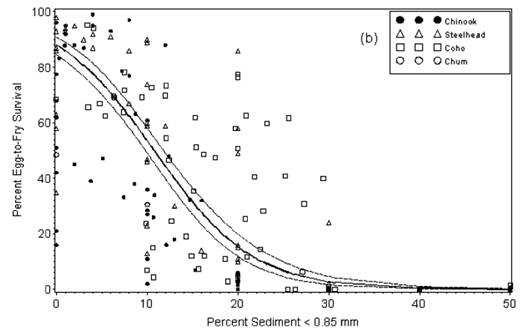
\includegraphics{images/image005.png}

}

\caption{\label{fig-1}An example of a stressor-response function for
Pacific salmon from Jensen et al. (2009) shows the relationship between
a stressor (percent fine sediment) on the x-axis and the biological
response (percent egg-to-fry survivorship) on the y-axis.}

\end{figure}

There are many types of stressor-response functions, including linear,
threshold, and non-linear ((Rosenfeld, 2017); (Larned \& Schallenberg,
2019)). Linear functions describe a simple, linear relationship between
the stressor and the response, with the response increasing or
decreasing at a constant rate as the stressor increases. Threshold
functions describe a breakpoint at which a stressor becomes harmful,
beyond which the response increases rapidly. Non-linear functions
describe more complex relationships, with the response changing at
different rates as the stressor increases. The example provided in
Figure Figure~\ref{fig-1} shows a customized non-linear
stressor-response function fit to empirical data (reference points).
Stressors do not always act independently ((Schäfer \& Piggott, 2018);
(Jarvis et al., 2023)), and it is also possible to include interactions
among variables in stressor-response functions, such as the risk of
exposure to a harmful pathogen being temperature dependent.

For a more in-depth discussion on the foundations of stressor-response
functions, refer to the following resources:

\begin{itemize}
\tightlist
\item
  (Rosenfeld et al., 2024)\textbf{; (Jarvis et al., 2023)}: Conceptual
  overviews of stressor-response functions as a generalizable model for
  context dependence. This paper provides a valuable overview to
  conceptualize stressors as a mechanism to characterize the state of a
  system and ecological process. Jarvis et al.~2023 also outline common
  forms of stressor-response functions and key considerations for the
  creation of a stressor-response function from empirical data.
\item
  (Piet et al., 2021): \emph{A roadmap towards quantitative cumulative
  impact assessments: Every step of the way}. Provides an important
  roadmap for working groups to consider linkages between land-use
  activities, resulting ecosystem pressures, functional linkages in
  space and time (exposure) and the consideration of endpoints to target
  study systems.
\item
  \textbf{Incorporating Indigenous Knowledge}: In many instances,
  stressor-response functions may be developed through expert opinion
  from local communities based on value systems. Where appropriate,
  working groups may include a customized stressor-response function to
  represent potential risks and values based on traditional knowledge
  systems and expert opinion. Refer to (Houde, 2007) and (Alexander et
  al., 2019) for further discussion. Examples of many other values-based
  Indigenous-led cumulative effects management programs exist across
  Canada.
\end{itemize}

\bookmarksetup{startatroot}

\hypertarget{modelling-pathways-and-assessment-endpoints}{%
\chapter{Modelling Pathways and Assessment
Endpoints}\label{modelling-pathways-and-assessment-endpoints}}

The CEMPRA framework offers several different modelling options and
assessment endpoints to choose from (Figure~\ref{fig-figure2}). The
specific endpoint to use will depend on the application, data
availability, and overall objectives of the assessment. In the following
section, we will describe stressor-response functions and the simplified
``Joe Model'' that combines the effects of multiple stressors on the
single adult life stage. We will also discuss the integrated life cycle
model, which links stressors to vital rates for multiple life history
stages to project productivity and capacity of the target system.
Although assessment endpoints differ between the modelling streams, they
all rely on stressor-response functions as the central theme of the
modelling process.

\begin{figure}

{\centering 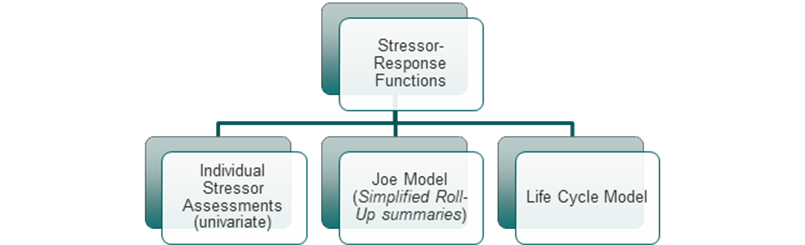
\includegraphics{images/image006.png}

}

\caption{\label{fig-figure2}Overview of alternative assessment endpoints
within the CEMPRA framework.}

\end{figure}

\hypertarget{individual-stressor-assessments-univariate}{%
\section{Individual Stressor Assessments
(univariate)}\label{individual-stressor-assessments-univariate}}

When setting up a cumulative effects model, it is often essential to
visualize the spatial distribution of stressor magnitudes. The CEMPRA
visual interface is organized around a centralized map interface (see
Section 6), which allows users to flip through stressors individually to
produce univariate heatmaps (choropleth maps) of each stressor
distribution (see Figure~\ref{fig-figure3}). These summaries are simple
yet useful to provide a general overview of the study area, stressors,
and associated stressor-response functions. The visual interpretation of
univariate stressor summaries is largely qualitative. The intent is to
visually identify hotspots and/or determine which stressors are high
everywhere or low everywhere based on the input stressor magnitude data
for each location and the corresponding predicted habitat capacity.

\begin{figure}

{\centering 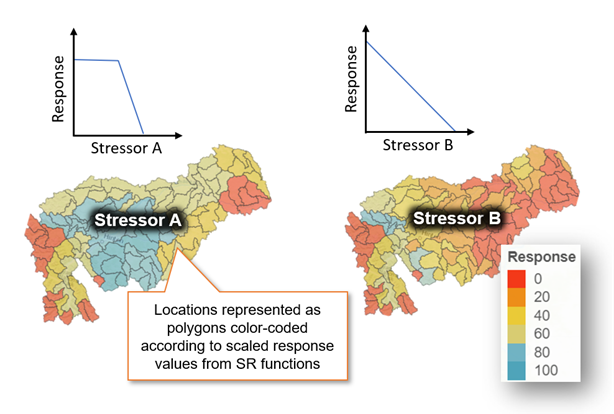
\includegraphics{images/image007.png}

}

\caption{\label{fig-figure3}Example of single (univariate) assessment of
stressors and stressor-response relationship for hypothetical stressors
A \& B with univariate heatmaps of predicted single-stressor habitat
capacity (``Response'' from 0-100\%) generated for the study area.}

\end{figure}

\hypertarget{joe-model-simplified-stressor-roll-up-summaries}{%
\section{Joe Model: Simplified Stressor Roll-up
Summaries}\label{joe-model-simplified-stressor-roll-up-summaries}}

The Joe Model component of the CEMPRA tool leverages the library of
stressor-response functions, defined and uploaded by the user, to
generate a simplified roll-up summary (cumulative effects score) across
multiple stressors. These summaries are simply the product of the scaled
response values (from 0 to 1, equivalent to 0-100\% of the system
carrying capacity for adults) of all stressors for each location
(Figure~\ref{fig-figure4}). Different stressors can be selected (or
omitted) from this summary depending on data availability or to
characterize different potential impact pathways.

In the Joe Model, the response component of each stressor-response
function (y-axis) is characterized broadly as the `Mean System Capacity'
of the target study system. `Mean System Capacity' specifically refers
to the adult carrying capacity since the basic Joe model is single-stage
and assumes that each stressor-response function is calibrated to the
adult system capacity; for example, even though in reality, it is
salmonid egg and fry survival that are directly impacted by high
Selenium concentrations, the effect of selenium dose will be scaled to
the impact on the adult population size in the Selenium
stressor-response function. This simplification of stage-structured
dynamics into a single life stage is one of the key features of the Joe
model that allows application to data-deficient species.

The calculated Mean System Capacity (Figure~\ref{fig-figure4}) is also
referred to as a ``cumulative effect score''. Although it can logically
be considered an estimate of adult carrying capacity as described above,
it also represents a scoring procedure for multiple stressors. In the
Joe Model summaries, the cumulative effect score across stressors is
calculated by multiplying the mean system capacity metrics together
(Figure~\ref{fig-figure4}). However, the model also offers the option
for users to custom-define the scoring algorithm (e.g., so that it is
not multiplicative; see Sandbox section), in which case it may no longer
represent carrying capacity. The Joe Model does not require the
weighting of individual stressors; since each stressor is scaled to a
maximum of 1, they are all weighed equally by default. By doing this,
the Joe Model avoids long-standing difficulties associated with
weighting impacts ((Walters, 1997)). In effect, the weights of stressors
are represented by the response value (0-1) associated with any given
stressor magnitude (Figure~\ref{fig-figure4}).

\begin{figure}

{\centering 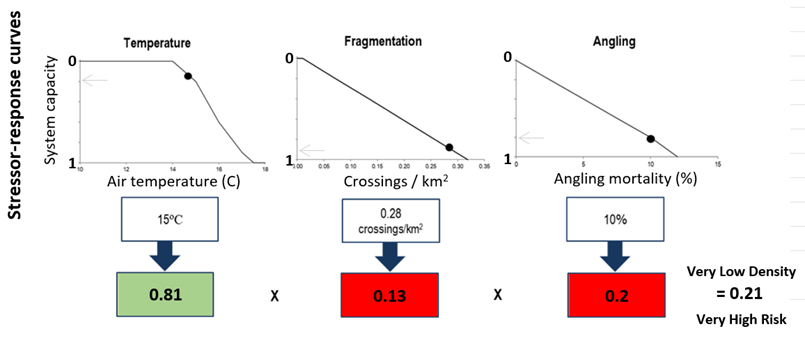
\includegraphics{images/image008.png}

}

\caption{\label{fig-figure4}Additive effect of multiple stressors in the
Joe Model. Figure modified from MacPherson et al., 2020.}

\end{figure}

The full implementation of the ``Joe Model'' extends this basic summary
to include stochastic simulations with uncertainty represented in both
the raw stressor values for each location and the response function
(described further in Section 5). These summaries are useful to
represent the risk of cumulative effects or current conditions as a
distribution rather than a fixed value.

\hypertarget{life-cycle-model}{%
\section{Life Cycle Model}\label{life-cycle-model}}

An integrated life cycle modelling framework is also included within the
CEMPRA tool to evaluate the effects of stressors on population-level
productivity and capacity (Figure~\ref{fig-figure5}). The embedded life
cycle modelling framework consists of a stage-structured matrix model
that allows users to link stressor-response functions to vital rates for
specific life stages (e.g., egg survivorship, fry capacity etc.), unlike
the Joe model, where the impact of stressors across multiple life stages
are integrated into a single stressor-response function linked to adult
capacity. The life cycle model estimates relative changes to
population-level productivity and capacity through simulations. A
flexible species profile input dataset is available so that users can
change values in the species profile to represent different study
systems with different life history stages or demographic parameters
(e.g., Athabasca Rainbow Trout, Chinook Salmon, etc.). See sections 6.4
and 7 for a detailed summary of the life cycle modelling framework
within the CEMPRA tool.

\begin{figure}

{\centering 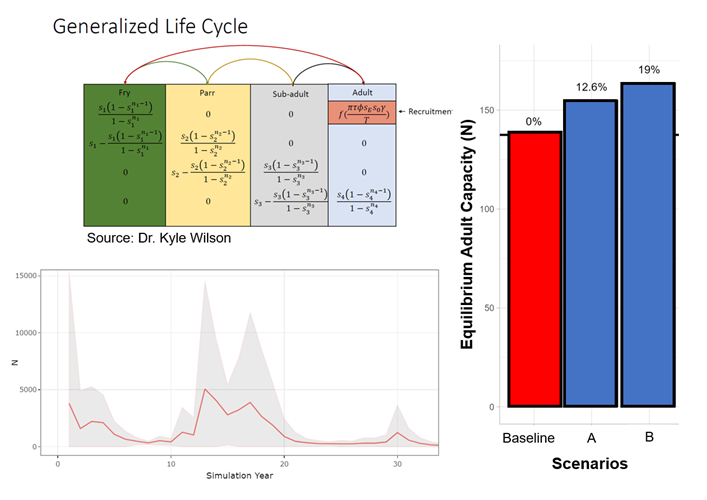
\includegraphics{images/image009.png}

}

\caption{\label{fig-figure5}Sample outputs from the Life Cycle Modelling
component of the CEMPRA tool.}

\end{figure}

\bookmarksetup{startatroot}

\hypertarget{initial-setup}{%
\chapter{Initial Setup}\label{initial-setup}}

There are two ways to interact with the CEMPRA (Joe Model): through the
R Shiny web application or directly using the stand alone CEMPRA R
package, which can be downloaded to the users personal computer.
Individuals unfamiliar with R can access the web application currently
available here:

\emph{The web version of the CEMPRA Tool}:
\url{https://essa.shinyapps.io/CEMPRAShiny/}

However, we strongly recommend that individuals familiar with R download
a local copy of the CEMPRA (Joe Model) Shiny application and run it on
their own computers through RStudio. Running the application from your
own computer reduces latency and other issues.

The CEMPRA framework is available as an R package and an R Shiny
application. All components of the project are freely available and open
source. Both the R package and the R Shiny application are freely
available for download from GitHub:

\emph{R package}: \url{https://github.com/essatech/CEMPRA/}

\emph{R Shiny application}:
\url{https://github.com/essatech/CEMPRAShiny}

\hypertarget{r-package}{%
\section{R-Package}\label{r-package}}

\begin{figure}

{\centering 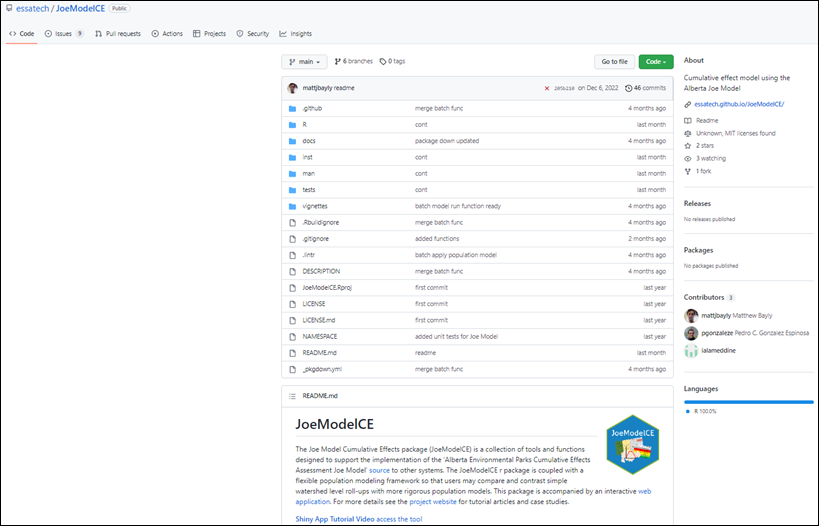
\includegraphics{images/image010.png}

}

\caption{\label{fig-figure6}CEMPRA package repository available on
GitHub (https://github.com/essatech/CEMPRA/).}

\end{figure}

The \emph{CEMPRA} package is part of a larger initiative to develop a
framework for modelling cumulative impacts to Species-at-Risk (SAR) to
guide recovery planning and adaptive management based on
stressor-response functions related to taxa-specific threats. This
framework allows users to generate models across a range of complexity
and data quality, treating stressor-response functions as modular
entities. The long-term vision is to build a library of
stressor-response functions to allow users to accelerate the transition
to quantitative modelling and adaptive management for Species at Risk
and to encourage the archiving of CEMPRA models along with Species at
Risk recovery strategies.

A quick start guide is provided below, but see Appendix D for tutorials
and function documentation.

\hypertarget{r-shiny-application}{%
\section{R Shiny Application}\label{r-shiny-application}}

\begin{figure}

{\centering 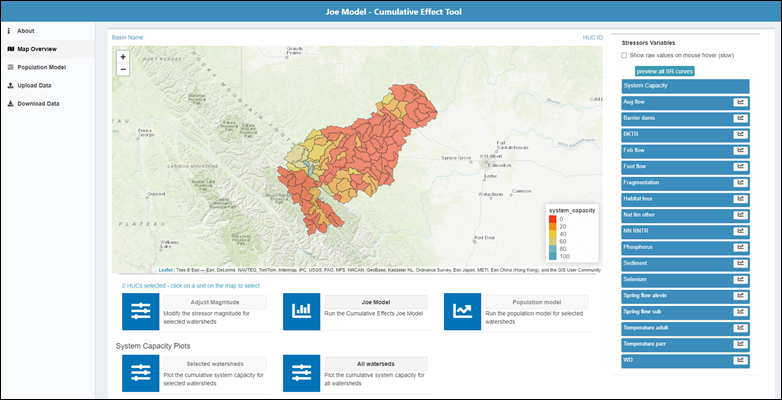
\includegraphics{images/image011.png}

}

\caption{\label{fig-figure7}Map Overview of results in the CEMPRA Shiny
web application.}

\end{figure}

The CEMPRA modelling tool includes the \emph{CEMPRA} R package, which is
accompanied by an interactive R Shiny web application
(https://essa.shinyapps.io/CEMPRAShiny; also available as the
stand-alone Shiny app). This application acts as a flexible,
user-friendly interface to interact with key components of the CEMPRA
tool. It accepts user inputs for stressor-response functions, stressor
magnitude, spatial units/polygons, and vital rates (for the life cycle
model portion). Results are easily mapped, summarized, and plotted
within the \textbf{Map Overview} page of the web application. Scenario
results generated from the tool (and the associated life cycle model)
can be exported directly from the application as an Excel spreadsheet
(.xlsx). See Section 5 for details on data inputs and Section 6 for a
complete walkthrough of the application.

\hypertarget{initial-setup-and-installation}{%
\section{Initial Setup and
Installation}\label{initial-setup-and-installation}}

Inexperienced R users can run the Joe Model directly through the web
application (\url{https://essa.shinyapps.io/CEMPRAShiny/}). However,
downloading and running the model directly in RStudio is recommended for
improved performance. Running the application locally (outside of
shinyapps.io) also guarantees data privacy. To run the application
locally, users must first have R and RStudio downloaded and installed on
their computers. The \emph{CEMPRA} R package
(\url{https://github.com/essatech/CEMPRA/}) and the local version of the
R Shiny web application (\url{https://github.com/essatech/CEMPRAShiny})
can be downloaded from GitHub.

To install R and RStudio on your computer:

\begin{enumerate}
\def\labelenumi{\arabic{enumi}.}
\tightlist
\item
  Go to the R website (\url{https://cran.r-project.org/}) and follow the
  instructions to download the latest version of R for your operating
  system (Windows, Mac, or Linux).
\item
  Once the download is complete, double-click (open) the installer file
  and follow the prompts to install R on your computer.
\item
  To open and run R scripts (files ending in .R), you can use RStudio, a
  popular Integrated Development Environment (IDE) for R. You can
  download the latest version of RStudio from:
  \url{https://rstudio.com/products/rstudio/download/}.
\end{enumerate}

To install the \emph{CEMPRA} R package on your computer:

\begin{enumerate}
\def\labelenumi{\arabic{enumi}.}
\tightlist
\item
  Download the \emph{CEMPRA} R package from GitHub
  (\url{https://github.com/essatech/CEMPRA/}) onto your computer by
  clicking the green ``Code'' button and selecting ``Download ZIP'' from
  the dropdown. Unzip the folder once the download is complete.
\item
  Install the \emph{CEMPRA} R Package. The easiest way to install the
  \emph{CEMPRA} package is from within RStudio using
  \texttt{remotes::install\_github()}. At this time, the package has not
  been published to CRAN, so the default \texttt{install.packages()}
  will not work for installing the \emph{CEMPRA} package. Instead, use
  the \texttt{remotes} package (or \texttt{devtools}). Open RStudio and
  install the \texttt{remotes} package using the
  \texttt{install.packages("remotes")} command in the Console. Next,
  install the \emph{CEMPRA} package from GitHub using the following
  commands in the Console:
\end{enumerate}

\begin{Shaded}
\begin{Highlighting}[]
\FunctionTok{install.packages}\NormalTok{(}\StringTok{"remotes"}\NormalTok{)}
\FunctionTok{library}\NormalTok{(remotes)}
\NormalTok{remotes}\SpecialCharTok{::}\FunctionTok{install\_github}\NormalTok{(}\StringTok{"essatech/CEMPRA"}\NormalTok{)}
\end{Highlighting}
\end{Shaded}

Once installed, use the \texttt{library(CEMPRA)} command to call the
\emph{CEMPRA} package into RStudio. You should only have to do the above
steps once on your computer.

\begin{figure}

{\centering 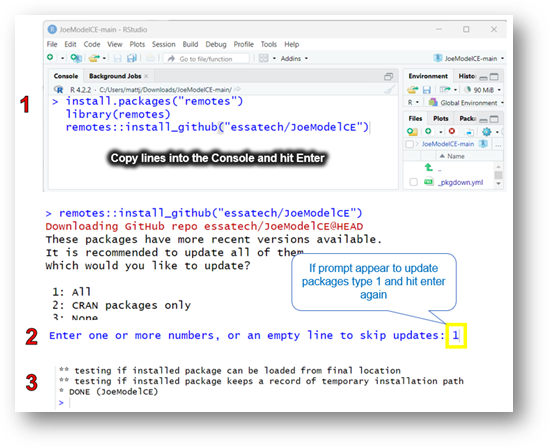
\includegraphics{images/image015.png}

}

\caption{\label{fig-picture45}Graphical user interface, text,
application, email. Description automatically generated.}

\end{figure}

\textbf{To access the raw code and example data for the R Shiny
application:}

\begin{enumerate}
\def\labelenumi{\arabic{enumi}.}
\item
  Download the \emph{CEMPRAShiny} repository from GitHub
  (\url{https://github.com/essatech/CEMPRAShiny}) onto your computer by
  clicking the green ``Code'' button and selecting ``Download ZIP'' from
  the dropdown. Unzip the folder once the download is complete.
\item
  Open the .Rproj file in R-Studio by double-clicking on it.
\end{enumerate}

\begin{figure}

{\centering 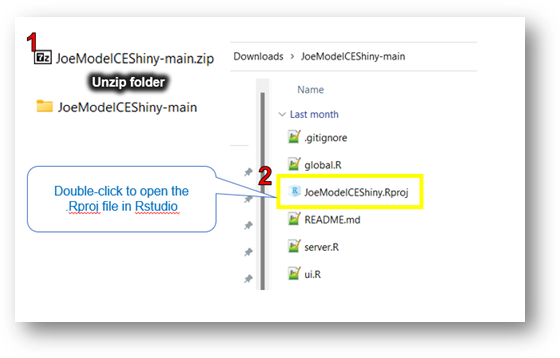
\includegraphics{images/image017.png}

}

\caption{\label{fig-picture48}Graphical user interface, application.
Description automatically generated.}

\end{figure}

\begin{enumerate}
\def\labelenumi{\arabic{enumi}.}
\setcounter{enumi}{2}
\tightlist
\item
  Open a script called global.R by double-clicking on it in the bottom
  right corner. Next, click the `Install' link on the yellow banner to
  install additional dependencies. Once complete, click the green arrow
  labelled `Run App' to launch the application.
\end{enumerate}

\begin{figure}

{\centering 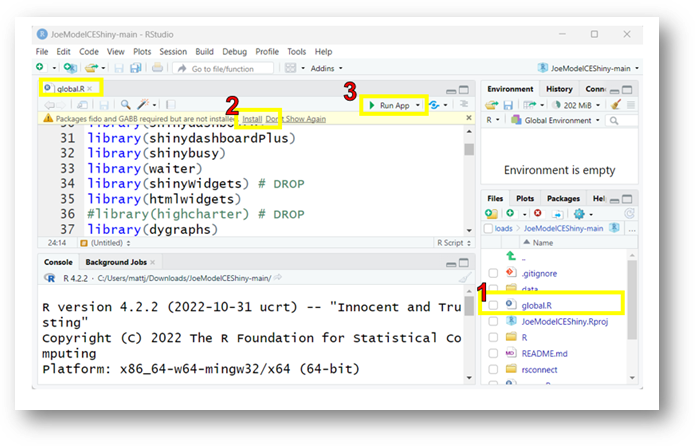
\includegraphics{images/image018.png}

}

\caption{\label{fig-picture47}Graphical user interface, text,
application. Description automatically generated.}

\end{figure}

Within the \emph{CEMPRAShiny} repository, example datasets are stored in
the ``demo'' subfolder within the ``data'' folder:

\url{https://github.com/essatech/CEMPRAShiny/tree/main/data/demo}

You only need to do the above steps once on your computer. Next time you
need to launch the application, simply click on the CEMPRAShiny.Rproj
file to open it in R Studio, then click on the green `Run App' button or
simply type `shiny::runApp()' in the console to launch the application.

\textbf{(Advanced) Using Windows command line to clone a GitHub
repository:}

For users comfortable using the command line who wish to contribute to
the project, GitHub repositories can be quickly cloned into a local
directory using this alternative method:

\emph{Note: Prior to using Git commands in the command line, you must
download and install Git on your computer
(\href{https://github.com/git-guides/install-git}{link}).}

\begin{enumerate}
\def\labelenumi{\arabic{enumi}.}
\item
  Navigate to the desired GitHub repository (\emph{CEMPRA} R package:
  \url{https://github.com/essatech/CEMPRA/}; \emph{CEMPRAShiny}
  application: \url{https://github.com/essatech/CEMPRAShiny}).
\item
  Click the green ``Code'' button and copy the URL from the HTTPS tab.
\item
  Open the Windows Command Prompt window on your computer. Set your
  working directory using the following command:
\end{enumerate}

\begin{Shaded}
\begin{Highlighting}[]
\BuiltInTok{cd}\NormalTok{ “}\OperatorTok{\textless{}}\NormalTok{file path}\OperatorTok{\textgreater{}}\NormalTok{”}
\end{Highlighting}
\end{Shaded}

\begin{enumerate}
\def\labelenumi{\arabic{enumi}.}
\setcounter{enumi}{3}
\tightlist
\item
  Next, use the git clone command to clone the GitHub repository into a
  folder in your working directory. For example:
\end{enumerate}

\begin{Shaded}
\begin{Highlighting}[]
\FunctionTok{git}\NormalTok{ clone https://github.com/essatech/CEMPRA.git}
\end{Highlighting}
\end{Shaded}

\bookmarksetup{startatroot}

\hypertarget{data-inputs}{%
\chapter{Data Inputs}\label{data-inputs}}

A working example of all data inputs can be downloaded from a `demo'
directory with the CEMPRAShiny project repository:
\href{https://github.com/essatech/CEMPRAShiny/tree/main/data/demo}{CEMPRAShiny
demo}.

Download the repository locally and navigate to the demo folder:
.\CEMPRAShiny-main\data\demo:

\begin{itemize}
\tightlist
\item
  stressor\_response\_demo.xlsx
\item
  stressor\_magnitude\_demo.xlsx
\item
  watersheds.gpkg
\item
  life cycles.csv
\end{itemize}

\hypertarget{stressor-response-workbook}{%
\section{Stressor-Response Workbook}\label{stressor-response-workbook}}

\hypertarget{purpose-1}{%
\subsection{Purpose}\label{purpose-1}}

The stressor-response workbook contains all the stressor-response curves
applicable to a target study system (e.g., Athabasca Rainbow Trout).
These stressor-response curves are used within the CEMPRA (Joe Model)
tool to predict cumulative effects additively given stressor magnitude
values (discussed in the next section).

\hypertarget{layout}{%
\subsection{Layout}\label{layout}}

The stressor-response workbook is an Excel workbook containing all
stressor-response functions to be used in the CEMPRA (Joe Model). The
first worksheet contained within this Excel workbook must be titled
``Main''. This worksheet is used as a coversheet to describe and
organize each of the stressor-response curves. Subsequent worksheets
describe each of the stressor-response functions relevant to a
particular species, where each stressor-response function has its own
worksheet. Note that the spelling of the stressor name must be identical
between the ``Stressors'' column in the ``Main'' worksheet and the
worksheet title (on the bottom tab) for each stressor.

\emph{Work is currently underway to develop an online stressor-response
web database (a digital repository of stressor-response functions across
species, systems and geographic areas compiled across reference
literature}). As this database grows, functionality will be expanded to
automatically generate a stressor-response workbook of selected
stressors using the R-package (CEMPRA). See details in Appendix A.

\hypertarget{main-worksheet}{%
\subsubsection{Main Worksheet}\label{main-worksheet}}

\begin{figure}

{\centering 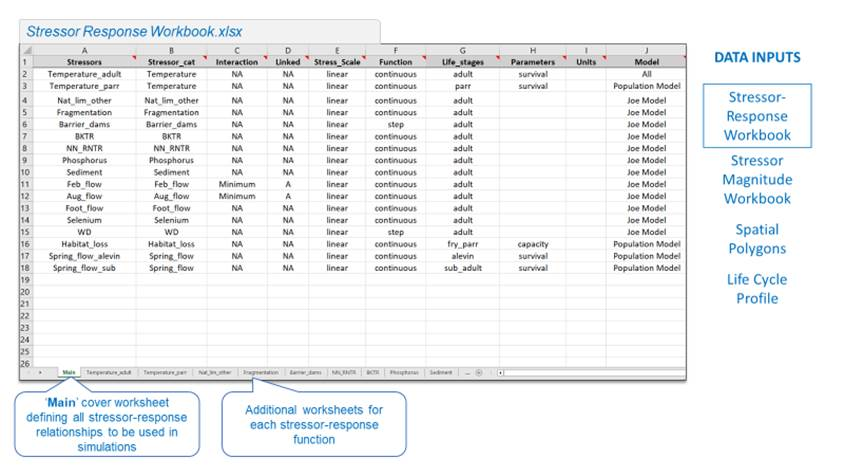
\includegraphics{images/image019.jpg}

}

\caption{\label{fig-main-worksheet}Main worksheet in the
Stressor-Response workbook.}

\end{figure}

Figure~\ref{fig-main-worksheet} shows the main worksheet in the
Stressor-Response workbook.

The purpose of the ``Main'' worksheet is to organize and summarize
stressor-response functions within the workbook. The columns within this
worksheet are set up as follows. Inputs must be diligently followed in
order for the code to work:

\hypertarget{individual-stressor-response-curve-worksheets}{%
\subsubsection{Individual Stressor-Response Curve
Worksheets}\label{individual-stressor-response-curve-worksheets}}

The remaining worksheets in the Stressor-response workbook are all used
to describe the relationships between raw stressor values (on the
x-axis) and the biological response (on the y-axis) (i.e., the
stressor-response data).

\begin{figure}

{\centering 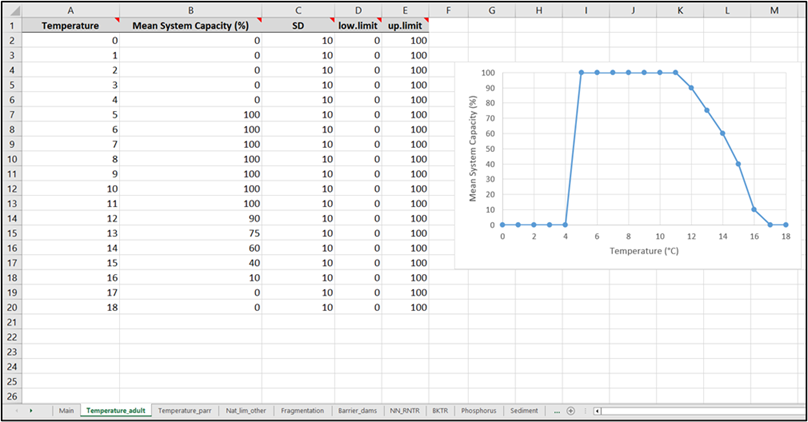
\includegraphics{images/image020.png}

}

\caption{\label{fig-individual-stressor}Example of an individual
stressor worksheet within the stressor response Excel workbook.}

\end{figure}

\begin{enumerate}
\def\labelenumi{\arabic{enumi}.}
\tightlist
\item
  Example of an individual stressor worksheet within the stressor
  response Excel workbook.
\end{enumerate}

Individual stressor worksheets within the stressor-response file contain
stressor-response curves for each of the stressor-response functions
outlined in the ``Main'' worksheet (one worksheet for each row). The
spelling of the worksheet name must exactly match the spelling of the
stressor on the `Main' worksheet. Additional rows can be added (as
needed) to increase the resolution and specify the shape of a complex
non-linear stressor response curve. Threshold stressor-response
functions or stressor-response functions with discrete values may have
relatively few rows.

\hypertarget{how-to-build-your-own-stressor-response-function}{%
\subsection{How to Build Your Own Stressor-Response
Function}\label{how-to-build-your-own-stressor-response-function}}

CEMPRA (Joe Model) users can either select pre-assembled
stressor-response functions or define their own stressor-response
functions for use in the model. A library is currently being developed
to host pre-assembled stressor-response functions and their associated
documentation (Appendix A). Users who develop their own
stressor-response functions are encouraged to fill out the appropriate
documentation for their function and upload it to this public
stressor-response library for future use (Appendix A). Please see
MacPherson et al.~(2018) and Rosenfeld et al.~2022 for further
discussion on fundamental considerations in the development of
customized stressor-response functions.

\hypertarget{methodology}{%
\subsubsection{Methodology}\label{methodology}}

Depending on data availability, stressor-response functions may be
developed from available empirical data, from the elicitation of experts
and stakeholders, or from existing literature.

\hypertarget{stressor-magnitude-file}{%
\section{Stressor Magnitude File}\label{stressor-magnitude-file}}

\hypertarget{purpose-2}{%
\subsection{Purpose}\label{purpose-2}}

The stressor magnitude file is an Excel worksheet which defines and
bounds each stressor within the individual locations (i.e., spatial
units) being assessed. Similar to the stressor-response functions,
stressor magnitude values are sampled across locations with
stochasticity. The stressor magnitude workbook is structured
accordingly, with data for each stressor and location entered into the
dataset in a long table format (as opposed to the standard wide table
format). Each row specifies a unique stressor for each unique location.
Therefore, the number of rows in this dataset should be equal to the
number of stressors multiplied by the number of locations. For each
simulation in the CEMPRA tool, values are sampled at random with
stochasticity for each stressor and location. For each year and batch
replicate, stressor magnitude values will be drawn from each normal (or
lognormal) distribution based on the Mean and SD (standard deviation)
and then further constrained based on the specified lower and upper
limits.

\begin{figure}

{\centering 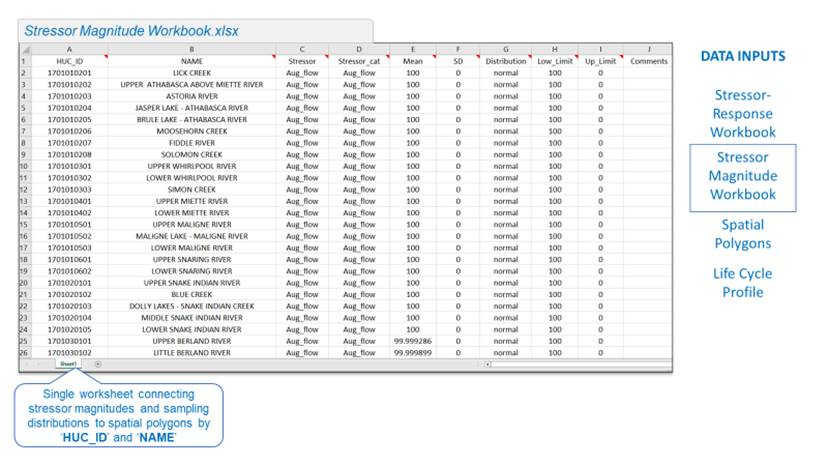
\includegraphics{images/image021.jpg}

}

\caption{\label{fig-stressor-magnitude}Example of a stressor magnitude
workbook.}

\end{figure}

\hypertarget{layout-1}{%
\subsection{Layout}\label{layout-1}}

Each row in the stressor magnitude workbook specifies a relationship
between a unique stressor and a unique location. Locations (discussed in
detail in the next section) are specified by a unique ID (HUC\_ID) and
NAME. The HUC\_ID column is a legacy from an older version of the Joe
Model that referenced Hydrological Unit Codes as ID values, but HUC\_ID
can be any set of unique IDs specified by the user for their spatial
units of interest. The NAME column can be blank but is included for
convenience since many users find it challenging to cross-reference ID
values between different datasets.

\hypertarget{assembling-your-own-stressor-magnitude-data}{%
\subsection{Assembling Your Own Stressor-Magnitude
Data}\label{assembling-your-own-stressor-magnitude-data}}

Data for stressor magnitude estimates can come from a variety of
sources, including GIS data, modelled data, field data, expert opinion,
regional trends, or estimates from the literature. When assembling your
own stressor magnitude data, stressor magnitudes and ranges will need to
be assigned to the individual locations (spatial units) being
represented in the model. Stressors within each location must be
assigned a magnitude, and distribution or the SD value must be set to 0
for simulations with no stochasticity. Within each spatial unit, users
can specify the mean value, standard deviation, distribution (normal or
lognormal), and upper and lower limits of each stressor, as discussed in
the previous section.

\begin{figure}

{\centering 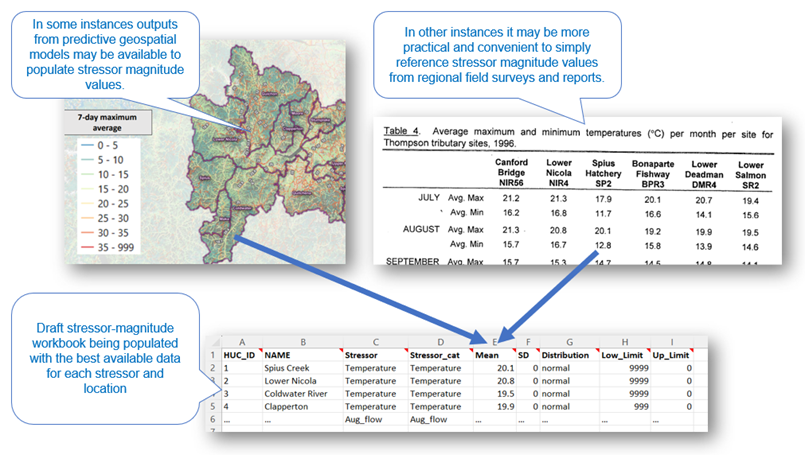
\includegraphics{images/image022.png}

}

\caption{\label{fig-stressor-magnitudes-values}Example of assigning
stressor magnitudes values (stream temperature) to spatial units
(locations).}

\end{figure}

Stressor magnitude values should be aggregated to locations to represent
location-averaged estimates. Locations can be split and aggregated as
needed such that each location represents averaged generalized
conditions.

\hypertarget{locations-spatial-polygons}{%
\section{Locations (Spatial
Polygons)}\label{locations-spatial-polygons}}

Locations are represented in the CEMPRA tool as spatial polygons.
Locations should be defined to reflect heterogeneity in stressor values
across the study area.

\begin{figure}

{\centering 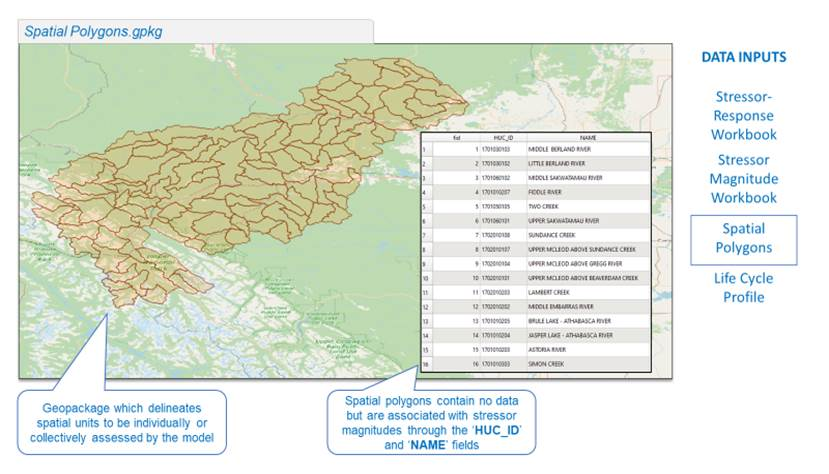
\includegraphics{images/image023.jpg}

}

\caption{\label{fig-spatial-polygons}Example of a spatial polygons
(locations) file and its associated attribute table with fields HUC\_ID
and NAME.}

\end{figure}

\hypertarget{life-cycles-profile}{%
\section{Life Cycles Profile}\label{life-cycles-profile}}

The life cycle profile (csv file) is an optional input applicable to
users who are interested in running the integrated life cycle model. The
life cycles profile file specifies all input parameters required to run
the life cycle model (e.g., number of stages, survival rates, fecundity,
etc.). The format of the life cycles profile is a generic template, but
once populated, it is used to parameterize the life cycle model for a
specific study system. Usually, this consists of a target population
(e.g., Athabasca Rainbow Trout, Nicola Basin Chinook Salmon, etc.).

\begin{figure}

{\centering 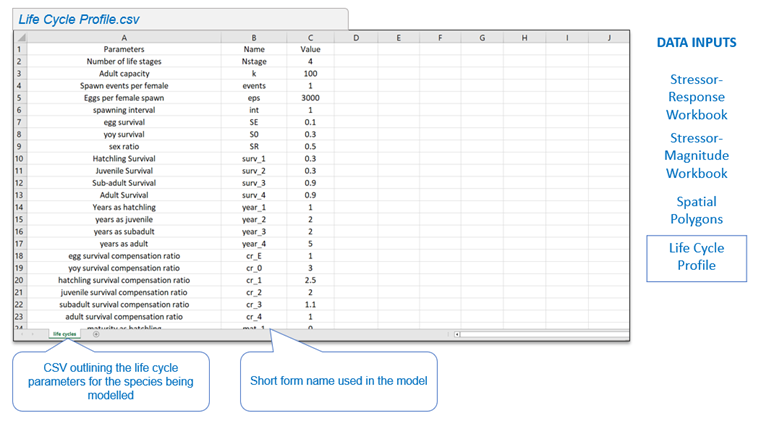
\includegraphics{images/image024.png}

}

\caption{\label{fig-life-cycles-profile}Example life cycles profile CSV
file.}

\end{figure}

A detailed discussion of the life cycles profile (csv file) is included
in Section 8.2 with accompanying background information. It's possible
to run the Joe Model and omit the life cycle model entirely. Therefore,
the life cycles profile csv should be considered as an optional input
for advanced use cases of the CEMPRA tool.

\bookmarksetup{startatroot}

\hypertarget{continue-here}{%
\chapter{CONTINUE HERE}\label{continue-here}}

There are two ways to interact with the CEMPRA (Joe Model): through the
R Shiny web application or directly using the stand alone CEMPRA R
package, which can be downloaded to the users personal computer.
Individuals unfamiliar with R can access the web application currently
available here:

\emph{The web version of the CEMPRA Tool}:
\url{https://essa.shinyapps.io/CEMPRAShiny/}

However, we strongly recommend that individuals familiar with R download
a local copy of the CEMPRA (Joe Model) Shiny application and run it on
their own computers through RStudio. Running the application from your
own computer reduces latency and other issues.

The CEMPRA framework is available as an R package and an R Shiny
application. All components of the project are freely available and open
source. Both the R package and the R Shiny application are freely
available for download from GitHub:

\emph{R package}: \url{https://github.com/essatech/CEMPRA/}

\emph{R Shiny application}:
\url{https://github.com/essatech/CEMPRAShiny}

\hypertarget{r-package-1}{%
\section{R-Package}\label{r-package-1}}

\begin{figure}

{\centering 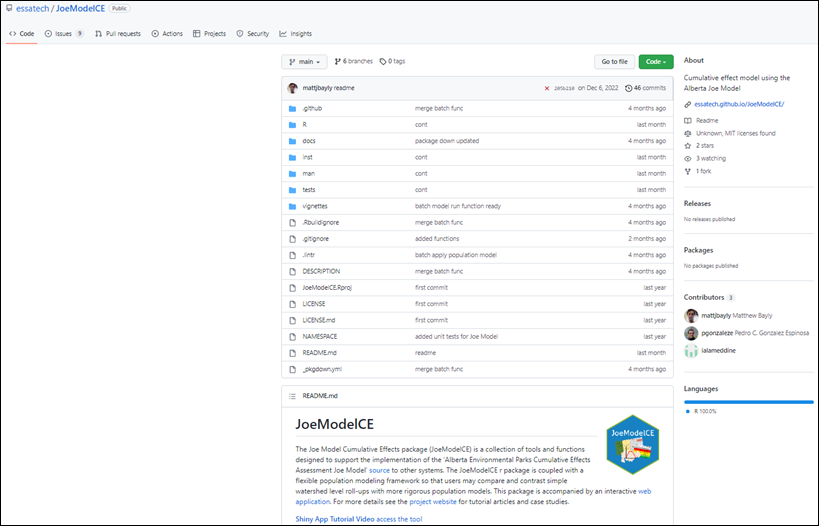
\includegraphics{images/image010.png}

}

\caption{\label{fig-figure6}CEMPRA package repository available on
GitHub (https://github.com/essatech/CEMPRA/).}

\end{figure}

The \emph{CEMPRA} package is part of a larger initiative to develop a
framework for modelling cumulative impacts to Species-at-Risk (SAR) to
guide recovery planning and adaptive management based on
stressor-response functions related to taxa-specific threats. This
framework allows users to generate models across a range of complexity
and data quality, treating stressor-response functions as modular
entities. The long-term vision is to build a library of
stressor-response functions to allow users to accelerate the transition
to quantitative modelling and adaptive management for Species at Risk
and to encourage the archiving of CEMPRA models along with Species at
Risk recovery strategies.

A quick start guide is provided below, but see Appendix D for tutorials
and function documentation.

\hypertarget{r-shiny-application-1}{%
\section{R Shiny Application}\label{r-shiny-application-1}}

\begin{figure}

{\centering 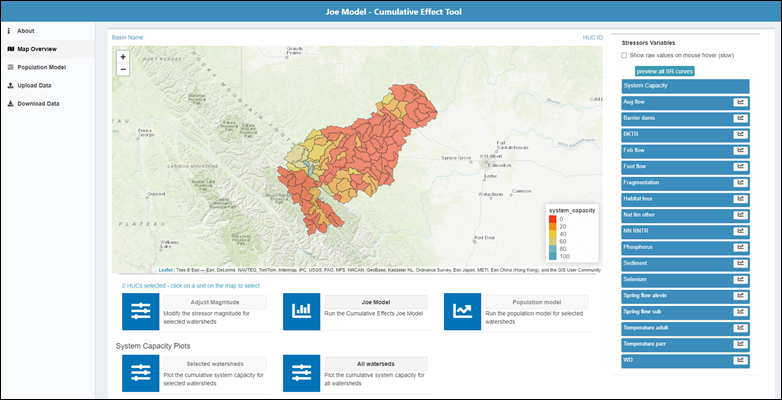
\includegraphics{images/image011.png}

}

\caption{Map Overview of results in the CEMPRA Shiny web application.}

\end{figure}

The CEMPRA modelling tool includes the \emph{CEMPRA} R package, which is
accompanied by an interactive R Shiny web application
(https://essa.shinyapps.io/CEMPRAShiny; also available as the
stand-alone Shiny app). This application acts as a flexible,
user-friendly interface to interact with key components of the CEMPRA
tool. It accepts user inputs for stressor-response functions, stressor
magnitude, spatial units/polygons, and vital rates (for the life cycle
model portion). Results are easily mapped, summarized, and plotted
within the \textbf{Map Overview} page of the web application. Scenario
results generated from the tool (and the associated life cycle model)
can be exported directly from the application as an Excel spreadsheet
(.xlsx). See Section 5 for details on data inputs and Section 6 for a
complete walkthrough of the application.

\hypertarget{initial-setup-and-installation-1}{%
\section{Initial Setup and
Installation}\label{initial-setup-and-installation-1}}

Inexperienced R users can run the Joe Model directly through the web
application (\url{https://essa.shinyapps.io/CEMPRAShiny/}). However,
downloading and running the model directly in RStudio is recommended for
improved performance. Running the application locally (outside of
shinyapps.io) also guarantees data privacy. To run the application
locally, users must first have R and RStudio downloaded and installed on
their computers. The \emph{CEMPRA} R package
(\url{https://github.com/essatech/CEMPRA/}) and the local version of the
R Shiny web application (\url{https://github.com/essatech/CEMPRAShiny})
can be downloaded from GitHub.

To install R and RStudio on your computer:

\begin{enumerate}
\def\labelenumi{\arabic{enumi}.}
\tightlist
\item
  Go to the R website (\url{https://cran.r-project.org/}) and follow the
  instructions to download the latest version of R for your operating
  system (Windows, Mac, or Linux).
\item
  Once the download is complete, double-click (open) the installer file
  and follow the prompts to install R on your computer.
\item
  To open and run R scripts (files ending in .R), you can use RStudio, a
  popular Integrated Development Environment (IDE) for R. You can
  download the latest version of RStudio from:
  \url{https://rstudio.com/products/rstudio/download/}.
\end{enumerate}

To install the \emph{CEMPRA} R package on your computer:

\begin{enumerate}
\def\labelenumi{\arabic{enumi}.}
\tightlist
\item
  Download the \emph{CEMPRA} R package from GitHub
  (\url{https://github.com/essatech/CEMPRA/}) onto your computer by
  clicking the green ``Code'' button and selecting ``Download ZIP'' from
  the dropdown. Unzip the folder once the download is complete.
\item
  Install the \emph{CEMPRA} R Package. The easiest way to install the
  \emph{CEMPRA} package is from within RStudio using
  \texttt{remotes::install\_github()}. At this time, the package has not
  been published to CRAN, so the default \texttt{install.packages()}
  will not work for installing the \emph{CEMPRA} package. Instead, use
  the \texttt{remotes} package (or \texttt{devtools}). Open RStudio and
  install the \texttt{remotes} package using the
  \texttt{install.packages("remotes")} command in the Console. Next,
  install the \emph{CEMPRA} package from GitHub using the following
  commands in the Console:
\end{enumerate}

\begin{Shaded}
\begin{Highlighting}[]
\FunctionTok{install.packages}\NormalTok{(}\StringTok{"remotes"}\NormalTok{)}
\FunctionTok{library}\NormalTok{(remotes)}
\NormalTok{remotes}\SpecialCharTok{::}\FunctionTok{install\_github}\NormalTok{(}\StringTok{"essatech/CEMPRA"}\NormalTok{)}
\end{Highlighting}
\end{Shaded}

Once installed, use the \texttt{library(CEMPRA)} command to call the
\emph{CEMPRA} package into RStudio. You should only have to do the above
steps once on your computer.

\begin{figure}

{\centering 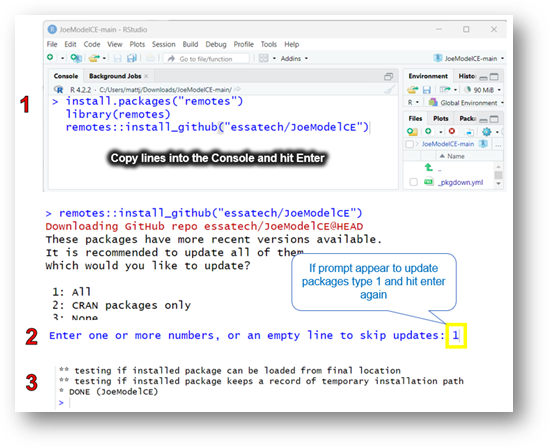
\includegraphics{images/image015.png}

}

\caption{Graphical user interface, text, application, email. Description
automatically generated.}

\end{figure}

\textbf{To access the raw code and example data for the R Shiny
application:}

\begin{enumerate}
\def\labelenumi{\arabic{enumi}.}
\item
  Download the \emph{CEMPRAShiny} repository from GitHub
  (\url{https://github.com/essatech/CEMPRAShiny}) onto your computer by
  clicking the green ``Code'' button and selecting ``Download ZIP'' from
  the dropdown. Unzip the folder once the download is complete.
\item
  Open the .Rproj file in R-Studio by double-clicking on it.
\end{enumerate}

\begin{figure}

{\centering 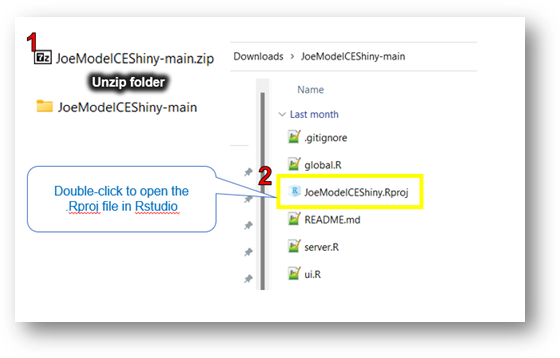
\includegraphics{images/image017.png}

}

\caption{Graphical user interface, application. Description
automatically generated.}

\end{figure}

\begin{enumerate}
\def\labelenumi{\arabic{enumi}.}
\setcounter{enumi}{2}
\tightlist
\item
  Open a script called global.R by double-clicking on it in the bottom
  right corner. Next, click the `Install' link on the yellow banner to
  install additional dependencies. Once complete, click the green arrow
  labelled `Run App' to launch the application.
\end{enumerate}

\begin{figure}

{\centering 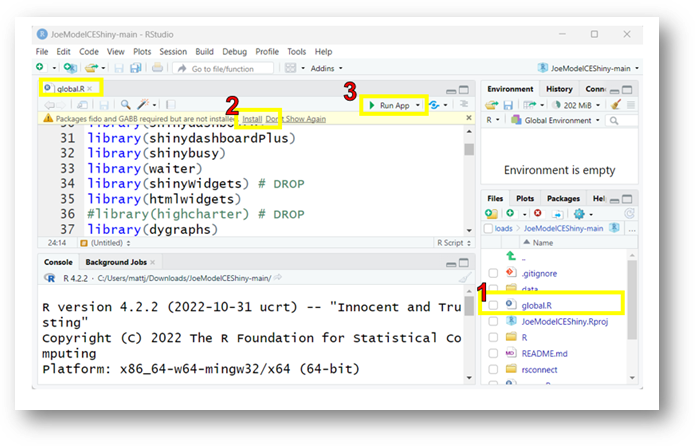
\includegraphics{images/image018.png}

}

\caption{Graphical user interface, text, application. Description
automatically generated.}

\end{figure}

Within the \emph{CEMPRAShiny} repository, example datasets are stored in
the ``demo'' subfolder within the ``data'' folder:

\url{https://github.com/essatech/CEMPRAShiny/tree/main/data/demo}

You only need to do the above steps once on your computer. Next time you
need to launch the application, simply click on the CEMPRAShiny.Rproj
file to open it in R Studio, then click on the green `Run App' button or
simply type `shiny::runApp()' in the console to launch the application.

\textbf{(Advanced) Using Windows command line to clone a GitHub
repository:}

For users comfortable using the command line who wish to contribute to
the project, GitHub repositories can be quickly cloned into a local
directory using this alternative method:

\emph{Note: Prior to using Git commands in the command line, you must
download and install Git on your computer
(\href{https://github.com/git-guides/install-git}{link}).}

\begin{enumerate}
\def\labelenumi{\arabic{enumi}.}
\item
  Navigate to the desired GitHub repository (\emph{CEMPRA} R package:
  \url{https://github.com/essatech/CEMPRA/}; \emph{CEMPRAShiny}
  application: \url{https://github.com/essatech/CEMPRAShiny}).
\item
  Click the green ``Code'' button and copy the URL from the HTTPS tab.
\item
  Open the Windows Command Prompt window on your computer. Set your
  working directory using the following command:
\end{enumerate}

\begin{Shaded}
\begin{Highlighting}[]
\BuiltInTok{cd}\NormalTok{ “}\OperatorTok{\textless{}}\NormalTok{file path}\OperatorTok{\textgreater{}}\NormalTok{”}
\end{Highlighting}
\end{Shaded}

\begin{enumerate}
\def\labelenumi{\arabic{enumi}.}
\setcounter{enumi}{3}
\tightlist
\item
  Next, use the git clone command to clone the GitHub repository into a
  folder in your working directory. For example:
\end{enumerate}

\begin{Shaded}
\begin{Highlighting}[]
\FunctionTok{git}\NormalTok{ clone https://github.com/essatech/CEMPRA.git}
\end{Highlighting}
\end{Shaded}

\bookmarksetup{startatroot}

\hypertarget{initial-setup-1}{%
\chapter{Initial Setup}\label{initial-setup-1}}

There are two ways to interact with the CEMPRA (Joe Model): through the
R Shiny web application or directly using the stand alone CEMPRA R
package, which can be downloaded to the users personal computer.
Individuals unfamiliar with R can access the web application currently
available here:

\emph{The web version of the CEMPRA Tool}:
\url{https://essa.shinyapps.io/CEMPRAShiny/}

However, we strongly recommend that individuals familiar with R download
a local copy of the CEMPRA (Joe Model) Shiny application and run it on
their own computers through RStudio. Running the application from your
own computer reduces latency and other issues.

The CEMPRA framework is available as an R package and an R Shiny
application. All components of the project are freely available and open
source. Both the R package and the R Shiny application are freely
available for download from GitHub:

\emph{R package}: \url{https://github.com/essatech/CEMPRA/}

\emph{R Shiny application}:
\url{https://github.com/essatech/CEMPRAShiny}

\hypertarget{r-package-2}{%
\section{R-Package}\label{r-package-2}}

\begin{figure}

{\centering 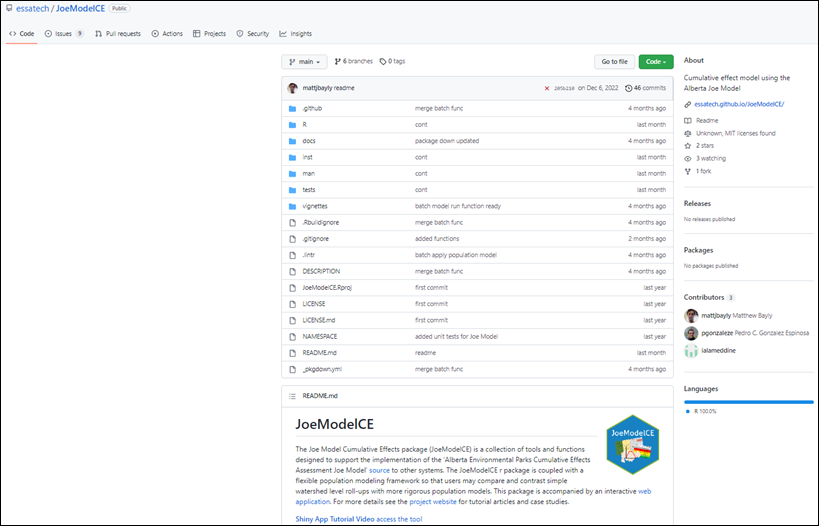
\includegraphics{images/image010.png}

}

\caption{\label{fig-figure6}CEMPRA package repository available on
GitHub (https://github.com/essatech/CEMPRA/).}

\end{figure}

The \emph{CEMPRA} package is part of a larger initiative to develop a
framework for modelling cumulative impacts to Species-at-Risk (SAR) to
guide recovery planning and adaptive management based on
stressor-response functions related to taxa-specific threats. This
framework allows users to generate models across a range of complexity
and data quality, treating stressor-response functions as modular
entities. The long-term vision is to build a library of
stressor-response functions to allow users to accelerate the transition
to quantitative modelling and adaptive management for Species at Risk
and to encourage the archiving of CEMPRA models along with Species at
Risk recovery strategies.

A quick start guide is provided below, but see Appendix D for tutorials
and function documentation.

\hypertarget{r-shiny-application-2}{%
\section{R Shiny Application}\label{r-shiny-application-2}}

\begin{figure}

{\centering 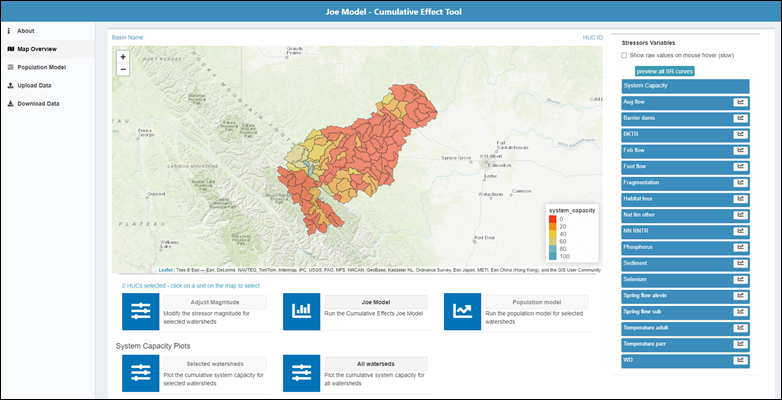
\includegraphics{images/image011.png}

}

\caption{\label{fig-figure7}Map Overview of results in the CEMPRA Shiny
web application.}

\end{figure}

The CEMPRA modelling tool includes the \emph{CEMPRA} R package, which is
accompanied by an interactive R Shiny web application
(https://essa.shinyapps.io/CEMPRAShiny; also available as the
stand-alone Shiny app). This application acts as a flexible,
user-friendly interface to interact with key components of the CEMPRA
tool. It accepts user inputs for stressor-response functions, stressor
magnitude, spatial units/polygons, and vital rates (for the life cycle
model portion). Results are easily mapped, summarized, and plotted
within the \textbf{Map Overview} page of the web application. Scenario
results generated from the tool (and the associated life cycle model)
can be exported directly from the application as an Excel spreadsheet
(.xlsx). See Section 5 for details on data inputs and Section 6 for a
complete walkthrough of the application.

\hypertarget{initial-setup-and-installation-2}{%
\section{Initial Setup and
Installation}\label{initial-setup-and-installation-2}}

Inexperienced R users can run the Joe Model directly through the web
application (\url{https://essa.shinyapps.io/CEMPRAShiny/}). However,
downloading and running the model directly in RStudio is recommended for
improved performance. Running the application locally (outside of
shinyapps.io) also guarantees data privacy. To run the application
locally, users must first have R and RStudio downloaded and installed on
their computers. The \emph{CEMPRA} R package
(\url{https://github.com/essatech/CEMPRA/}) and the local version of the
R Shiny web application (\url{https://github.com/essatech/CEMPRAShiny})
can be downloaded from GitHub.

To install R and RStudio on your computer:

\begin{enumerate}
\def\labelenumi{\arabic{enumi}.}
\tightlist
\item
  Go to the R website (\url{https://cran.r-project.org/}) and follow the
  instructions to download the latest version of R for your operating
  system (Windows, Mac, or Linux).
\item
  Once the download is complete, double-click (open) the installer file
  and follow the prompts to install R on your computer.
\item
  To open and run R scripts (files ending in .R), you can use RStudio, a
  popular Integrated Development Environment (IDE) for R. You can
  download the latest version of RStudio from:
  \url{https://rstudio.com/products/rstudio/download/}.
\end{enumerate}

To install the \emph{CEMPRA} R package on your computer:

\begin{enumerate}
\def\labelenumi{\arabic{enumi}.}
\tightlist
\item
  Download the \emph{CEMPRA} R package from GitHub
  (\url{https://github.com/essatech/CEMPRA/}) onto your computer by
  clicking the green ``Code'' button and selecting ``Download ZIP'' from
  the dropdown. Unzip the folder once the download is complete.
\item
  Install the \emph{CEMPRA} R Package. The easiest way to install the
  \emph{CEMPRA} package is from within RStudio using
  \texttt{remotes::install\_github()}. At this time, the package has not
  been published to CRAN, so the default \texttt{install.packages()}
  will not work for installing the \emph{CEMPRA} package. Instead, use
  the \texttt{remotes} package (or \texttt{devtools}). Open RStudio and
  install the \texttt{remotes} package using the
  \texttt{install.packages("remotes")} command in the Console. Next,
  install the \emph{CEMPRA} package from GitHub using the following
  commands in the Console:
\end{enumerate}

\begin{Shaded}
\begin{Highlighting}[]
\FunctionTok{install.packages}\NormalTok{(}\StringTok{"remotes"}\NormalTok{)}
\FunctionTok{library}\NormalTok{(remotes)}
\NormalTok{remotes}\SpecialCharTok{::}\FunctionTok{install\_github}\NormalTok{(}\StringTok{"essatech/CEMPRA"}\NormalTok{)}
\end{Highlighting}
\end{Shaded}

Once installed, use the \texttt{library(CEMPRA)} command to call the
\emph{CEMPRA} package into RStudio. You should only have to do the above
steps once on your computer.

\begin{figure}

{\centering 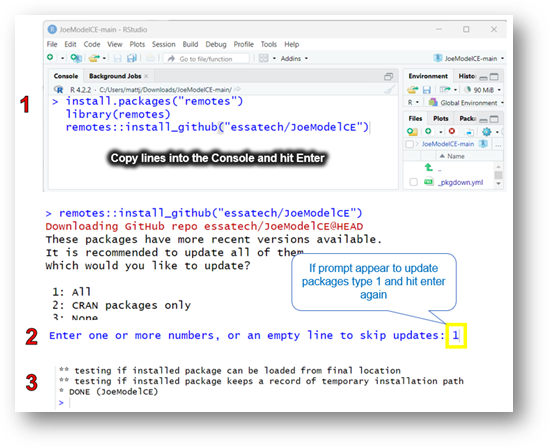
\includegraphics{images/image015.png}

}

\caption{\label{fig-picture45}Graphical user interface, text,
application, email. Description automatically generated.}

\end{figure}

\textbf{To access the raw code and example data for the R Shiny
application:}

\begin{enumerate}
\def\labelenumi{\arabic{enumi}.}
\item
  Download the \emph{CEMPRAShiny} repository from GitHub
  (\url{https://github.com/essatech/CEMPRAShiny}) onto your computer by
  clicking the green ``Code'' button and selecting ``Download ZIP'' from
  the dropdown. Unzip the folder once the download is complete.
\item
  Open the .Rproj file in R-Studio by double-clicking on it.
\end{enumerate}

\begin{figure}

{\centering 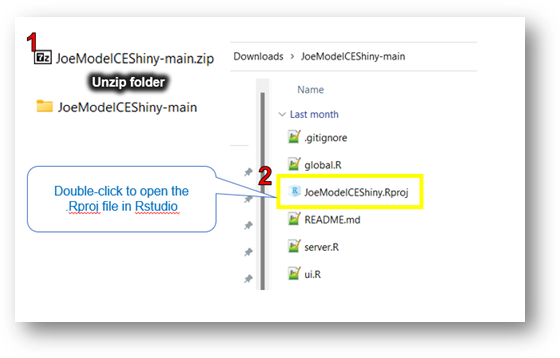
\includegraphics{images/image017.png}

}

\caption{\label{fig-picture48}Graphical user interface, application.
Description automatically generated.}

\end{figure}

\begin{enumerate}
\def\labelenumi{\arabic{enumi}.}
\setcounter{enumi}{2}
\tightlist
\item
  Open a script called global.R by double-clicking on it in the bottom
  right corner. Next, click the `Install' link on the yellow banner to
  install additional dependencies. Once complete, click the green arrow
  labelled `Run App' to launch the application.
\end{enumerate}

\begin{figure}

{\centering 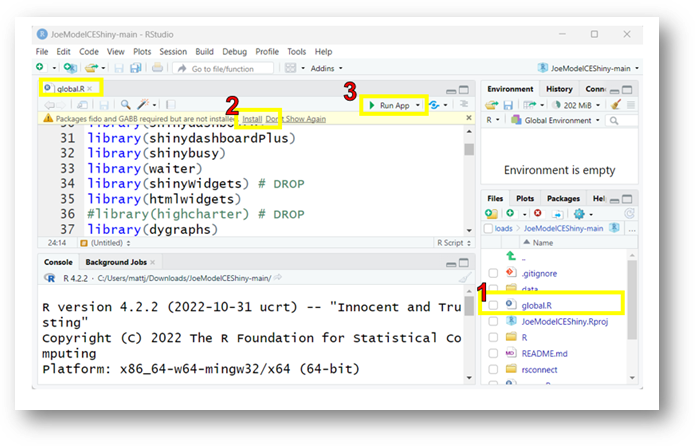
\includegraphics{images/image018.png}

}

\caption{\label{fig-picture47}Graphical user interface, text,
application. Description automatically generated.}

\end{figure}

Within the \emph{CEMPRAShiny} repository, example datasets are stored in
the ``demo'' subfolder within the ``data'' folder:

\url{https://github.com/essatech/CEMPRAShiny/tree/main/data/demo}

You only need to do the above steps once on your computer. Next time you
need to launch the application, simply click on the CEMPRAShiny.Rproj
file to open it in R Studio, then click on the green `Run App' button or
simply type `shiny::runApp()' in the console to launch the application.

\textbf{(Advanced) Using Windows command line to clone a GitHub
repository:}

For users comfortable using the command line who wish to contribute to
the project, GitHub repositories can be quickly cloned into a local
directory using this alternative method:

\emph{Note: Prior to using Git commands in the command line, you must
download and install Git on your computer
(\href{https://github.com/git-guides/install-git}{link}).}

\begin{enumerate}
\def\labelenumi{\arabic{enumi}.}
\item
  Navigate to the desired GitHub repository (\emph{CEMPRA} R package:
  \url{https://github.com/essatech/CEMPRA/}; \emph{CEMPRAShiny}
  application: \url{https://github.com/essatech/CEMPRAShiny}).
\item
  Click the green ``Code'' button and copy the URL from the HTTPS tab.
\item
  Open the Windows Command Prompt window on your computer. Set your
  working directory using the following command:
\end{enumerate}

\begin{Shaded}
\begin{Highlighting}[]
\BuiltInTok{cd}\NormalTok{ “}\OperatorTok{\textless{}}\NormalTok{file path}\OperatorTok{\textgreater{}}\NormalTok{”}
\end{Highlighting}
\end{Shaded}

\begin{enumerate}
\def\labelenumi{\arabic{enumi}.}
\setcounter{enumi}{3}
\tightlist
\item
  Next, use the git clone command to clone the GitHub repository into a
  folder in your working directory. For example:
\end{enumerate}

\begin{Shaded}
\begin{Highlighting}[]
\FunctionTok{git}\NormalTok{ clone https://github.com/essatech/CEMPRA.git}
\end{Highlighting}
\end{Shaded}

\bookmarksetup{startatroot}

\hypertarget{summary}{%
\chapter{Summary}\label{summary}}

In summary, this book has no content whatsoever.

\begin{Shaded}
\begin{Highlighting}[]
\DecValTok{1} \SpecialCharTok{+} \DecValTok{1}
\end{Highlighting}
\end{Shaded}

\begin{verbatim}
[1] 2
\end{verbatim}

\bookmarksetup{startatroot}

\hypertarget{references}{%
\chapter*{References}\label{references}}
\addcontentsline{toc}{chapter}{References}

\markboth{References}{References}

\hypertarget{refs}{}
\begin{CSLReferences}{1}{0}
\leavevmode\vadjust pre{\hypertarget{ref-alexander2019bridging}{}}%
Alexander, S. M., Provencher, J. F., Henri, D. A., Taylor, J. J.,
Lloren, J. I., Nanayakkara, L., et al. (2019). Bridging indigenous and
science-based knowledge in coastal and marine research, monitoring, and
management in canada. \emph{Environmental Evidence}, \emph{8}(1), 1--24.

\leavevmode\vadjust pre{\hypertarget{ref-halpern2013assumptions}{}}%
Halpern, B. S., \& Fujita, R. (2013). Assumptions, challenges, and
future directions in cumulative impact analysis. \emph{Ecosphere},
\emph{4}, 1--11.

\leavevmode\vadjust pre{\hypertarget{ref-houde2007six}{}}%
Houde, N. (2007). The six faces of traditional ecological knowledge:
Challenges and opportunities for canadian co-management arrangements.
\emph{Ecology and Society}, \emph{12}(2).

\leavevmode\vadjust pre{\hypertarget{ref-jarvis2023process}{}}%
Jarvis, L., Rosenfeld, J., Gonzalez-Espinosa, P., \& Enders, E. (2023).
A process framework for integrating stressor-response functions into
cumulative effects models. \emph{Science of the Total Environment},
\emph{XXX}, 167456.

\leavevmode\vadjust pre{\hypertarget{ref-jensen2009impact}{}}%
Jensen, D. W., Steel, E. A., Fullerton, A. H., \& Pess, G. R. (2009).
Impact of fine sediment on incubation survival of pacific salmon: A
meta-analysis of published studies. \emph{Reviews in Fisheries Science},
\emph{17}(3), 348--359. \url{https://doi.org/10.1080/10641260902716954}

\leavevmode\vadjust pre{\hypertarget{ref-larned2019stressor}{}}%
Larned, S. T., \& Schallenberg, M. (2019). Stressor-response
relationships and the prospective management of aquatic ecosystems.
\emph{New Zealand Journal of Marine and Freshwater Research}, \emph{53},
489--512.

\leavevmode\vadjust pre{\hypertarget{ref-macpherson2023prioritizing}{}}%
MacPherson, L. M., Reilly, J. R., Neufeld, K. R., Sullivan, M. G., Paul,
A. J., \& Johnston, F. D. (2023). Prioritizing bull trout recovery
actions using a novel cumulative effects modelling framework.
\emph{Fisheries Management and Ecology}, 1--17.

\leavevmode\vadjust pre{\hypertarget{ref-macpherson2020alberta}{}}%
MacPherson, L., Sullivan, M., Reilly, J., \& Paul, A. (2020).
\emph{Alberta's fisheries sustainability assessment: A guide to
assessing population status, and quantifying cumulative effects using
the joe modelling technique}. Canadian Science Advisory Secretariat
(CSAS).

\leavevmode\vadjust pre{\hypertarget{ref-pearsall2022nicola}{}}%
Pearsall, et al. (2022). \emph{Nicola watershed RAMS final report 2022:
Nicola basin chinook risk assessment final report. A process developed
with the nicola collaborative research and technical committee}.

\leavevmode\vadjust pre{\hypertarget{ref-piet2021roadmap}{}}%
Piet, G. J., Tamis, J. E., Volwater, J., Vries, P. de, Wal, J. T. van
der, \& Jongbloed, R. H. (2021). A roadmap towards quantitative
cumulative impact assessments: Every step of the way. \emph{Science of
The Total Environment}, \emph{784}, 146847.

\leavevmode\vadjust pre{\hypertarget{ref-pirotta2022understanding}{}}%
Pirotta, E., Thomas, L., Costa, D. P., Hall, A. J., Harris, C. M.,
Harwood, J., et al. (2022). Understanding the combined effects of
multiple stressors: A new perspective on a longstanding challenge.
\emph{Science of the Total Environment}, \emph{821}, 153322.

\leavevmode\vadjust pre{\hypertarget{ref-rosenfeld2017developing}{}}%
Rosenfeld, J. S. (2017). Developing flow--ecology relationships:
Implications of nonlinear biological responses for water management.
\emph{Freshwater Biology}, \emph{62}, 1305--1324.

\leavevmode\vadjust pre{\hypertarget{ref-rosenfeld2024determinants}{}}%
Rosenfeld, J. S., Ayllón, D., Grant, J. W., Naman, S. M., Post, J. R.,
Matte, J.-M., et al. (2024). Determinants of productive capacity for
stream salmonids. In J. Lobon-Cervia, P. Budy, \& R. Gresswell (Eds.),
\emph{Advances in the ecology of stream-dwelling salmonids} (pp. 1--12).
Springer Life Sciences.

\leavevmode\vadjust pre{\hypertarget{ref-schafer2018advancing}{}}%
Schäfer, R. B., \& Piggott, J. J. (2018). Advancing understanding and
prediction in multiple stressor research through a mechanistic basis for
null models. \emph{Global Change Biology}, \emph{24}, 1817--1826.

\leavevmode\vadjust pre{\hypertarget{ref-sullivan2017adaptive}{}}%
Sullivan, M. (2017). \emph{Adaptive management of athabasca rainbow
trout; cumulative effects modelling and potential management actions}.
Alberta Environment; Parks; Fisheries Management Branch.

\leavevmode\vadjust pre{\hypertarget{ref-walters1997challenges}{}}%
Walters, C. (1997). Challenges in adaptive management of riparian and
coastal ecosystems. \emph{Conservation Ecology {[}Online{]}},
\emph{1}(2), 1.

\end{CSLReferences}

\cleardoublepage
\phantomsection
\addcontentsline{toc}{part}{Appendices}
\appendix

\hypertarget{introduction-1}{%
\chapter{Introduction}\label{introduction-1}}

This is a book created from markdown and executable code.

See (\textbf{knuth84?}) for additional discussion of literate
programming.

\begin{Shaded}
\begin{Highlighting}[]
\DecValTok{1} \SpecialCharTok{+} \DecValTok{1}
\end{Highlighting}
\end{Shaded}

\begin{verbatim}
[1] 2
\end{verbatim}

\hypertarget{summary-1}{%
\chapter{Summary}\label{summary-1}}

In summary, this book has no content whatsoever.

\begin{Shaded}
\begin{Highlighting}[]
\DecValTok{1} \SpecialCharTok{+} \DecValTok{1}
\end{Highlighting}
\end{Shaded}

\begin{verbatim}
[1] 2
\end{verbatim}



\end{document}
